\documentclass[a4paper]{book}
\usepackage{a4wide}
\usepackage{makeidx}
\usepackage{fancyhdr}
\usepackage{graphicx}
\usepackage{multicol}
\usepackage{float}
\usepackage{listings}
\usepackage{color}
\usepackage{textcomp}
\usepackage{alltt}
\usepackage{times}
\usepackage{ifpdf}
\ifpdf
\usepackage[pdftex,
            pagebackref=true,
            colorlinks=true,
            linkcolor=blue,
            unicode
           ]{hyperref}
\else
\usepackage[ps2pdf,
            pagebackref=true,
            colorlinks=true,
            linkcolor=blue,
            unicode
           ]{hyperref}
\usepackage{pspicture}
\fi
\usepackage[utf8]{inputenc}
\usepackage{doxygen}
\lstset{language=C++,inputencoding=utf8,basicstyle=\footnotesize,breaklines=true,breakatwhitespace=true,tabsize=8,numbers=left }
\makeindex
\setcounter{tocdepth}{3}
\renewcommand{\footrulewidth}{0.4pt}
\begin{document}
\hypersetup{pageanchor=false}
\begin{titlepage}
\vspace*{7cm}
\begin{center}
{\Large openBibleViewer }\\
\vspace*{1cm}
{\large Generated by Doxygen 1.5.9}\\
\vspace*{0.5cm}
{\small Mon Dec 21 01:20:58 2009}\\
\end{center}
\end{titlepage}
\clearemptydoublepage
\pagenumbering{roman}
\tableofcontents
\clearemptydoublepage
\pagenumbering{arabic}
\hypersetup{pageanchor=true}
\chapter{Namespace Index}
\section{Namespace List}
Here is a list of all documented namespaces with brief descriptions:\begin{CompactList}
\item\contentsline{section}{\hyperlink{namespaceKoXml}{KoXml} }{\pageref{namespaceKoXml}}{}
\end{CompactList}

\chapter{Class Index}
\section{Class Hierarchy}
This inheritance list is sorted roughly, but not completely, alphabetically:\begin{DoxyCompactList}
\item \contentsline{section}{AboutDialog}{\pageref{classAboutDialog}}{}
\item \contentsline{section}{BibleDisplay}{\pageref{classBibleDisplay}}{}
\item \contentsline{section}{BibleDisplaySettings}{\pageref{classBibleDisplaySettings}}{}
\item \contentsline{section}{BiblePassageDialog}{\pageref{classBiblePassageDialog}}{}
\item \contentsline{section}{BibleQuote}{\pageref{classBibleQuote}}{}
\item \contentsline{section}{Chapter}{\pageref{structChapter}}{}
\item \contentsline{section}{DbgHelper}{\pageref{classDbgHelper}}{}
\item \contentsline{section}{DockWidget}{\pageref{classDockWidget}}{}
\begin{DoxyCompactList}
\item \contentsline{section}{BookDockWidget}{\pageref{classBookDockWidget}}{}
\item \contentsline{section}{BookmarksDockWidget}{\pageref{classBookmarksDockWidget}}{}
\item \contentsline{section}{ModuleDockWidget}{\pageref{classModuleDockWidget}}{}
\item \contentsline{section}{NotesDockWidget}{\pageref{classNotesDockWidget}}{}
\item \contentsline{section}{QuickJumpDockWidget}{\pageref{classQuickJumpDockWidget}}{}
\item \contentsline{section}{SearchResultDockWidget}{\pageref{classSearchResultDockWidget}}{}
\item \contentsline{section}{StrongDockWidget}{\pageref{classStrongDockWidget}}{}
\end{DoxyCompactList}
\item \contentsline{section}{GoTo}{\pageref{classGoTo}}{}
\item \contentsline{section}{History}{\pageref{classHistory}}{}
\item \contentsline{section}{Interface}{\pageref{classInterface}}{}
\begin{DoxyCompactList}
\item \contentsline{section}{AdvancedInterface}{\pageref{classAdvancedInterface}}{}
\item \contentsline{section}{SimpleInterface}{\pageref{classSimpleInterface}}{}
\item \contentsline{section}{StudyInterface}{\pageref{classStudyInterface}}{}
\end{DoxyCompactList}
\item \contentsline{section}{KoLZF}{\pageref{classKoLZF}}{}
\item \contentsline{section}{KoXmlHandler}{\pageref{classKoXmlHandler}}{}
\item \contentsline{section}{KoXmlInputSource}{\pageref{classKoXmlInputSource}}{}
\item \contentsline{section}{KoXmlNode}{\pageref{classKoXmlNode}}{}
\begin{DoxyCompactList}
\item \contentsline{section}{KoXmlDocument}{\pageref{classKoXmlDocument}}{}
\item \contentsline{section}{KoXmlDocumentType}{\pageref{classKoXmlDocumentType}}{}
\item \contentsline{section}{KoXmlElement}{\pageref{classKoXmlElement}}{}
\item \contentsline{section}{KoXmlText}{\pageref{classKoXmlText}}{}
\begin{DoxyCompactList}
\item \contentsline{section}{KoXmlCDATASection}{\pageref{classKoXmlCDATASection}}{}
\end{DoxyCompactList}
\end{DoxyCompactList}
\item \contentsline{section}{KoXmlNodeData}{\pageref{classKoXmlNodeData}}{}
\item \contentsline{section}{KoXmlPackedDocument}{\pageref{classKoXmlPackedDocument}}{}
\item \contentsline{section}{KoXmlPackedItem}{\pageref{classKoXmlPackedItem}}{}
\item \contentsline{section}{KoXmlVector$<$ T $>$}{\pageref{classKoXmlVector}}{}
\item \contentsline{section}{KoXmlWriter}{\pageref{classKoXmlWriter}}{}
\item \contentsline{section}{MainWindow}{\pageref{classMainWindow}}{}
\item \contentsline{section}{MarkCategories}{\pageref{classMarkCategories}}{}
\item \contentsline{section}{MarkList}{\pageref{classMarkList}}{}
\item \contentsline{section}{MdiForm}{\pageref{classMdiForm}}{}
\item \contentsline{section}{Module}{\pageref{classModule}}{}
\item \contentsline{section}{ModuleConfigDialog}{\pageref{classModuleConfigDialog}}{}
\item \contentsline{section}{ModuleDownloadDialog}{\pageref{classModuleDownloadDialog}}{}
\item \contentsline{section}{ModuleManager}{\pageref{classModuleManager}}{}
\item \contentsline{section}{ModuleSettings}{\pageref{classModuleSettings}}{}
\item \contentsline{section}{Notes}{\pageref{classNotes}}{}
\item \contentsline{section}{NotesEditor}{\pageref{classNotesEditor}}{}
\item \contentsline{section}{KoXmlWriter::Private}{\pageref{classKoXmlWriter_1_1Private}}{}
\item \contentsline{section}{SearchDialog}{\pageref{classSearchDialog}}{}
\item \contentsline{section}{SearchHit}{\pageref{classSearchHit}}{}
\item \contentsline{section}{SearchInfoDialog}{\pageref{classSearchInfoDialog}}{}
\item \contentsline{section}{SearchQuery}{\pageref{classSearchQuery}}{}
\item \contentsline{section}{SearchResult}{\pageref{classSearchResult}}{}
\item \contentsline{section}{Session}{\pageref{classSession}}{}
\item \contentsline{section}{Settings}{\pageref{classSettings}}{}
\item \contentsline{section}{SettingsDialog}{\pageref{classSettingsDialog}}{}
\item \contentsline{section}{SimpleModuleClass}{\pageref{classSimpleModuleClass}}{}
\begin{DoxyCompactList}
\item \contentsline{section}{Bible}{\pageref{classBible}}{}
\item \contentsline{section}{Strong}{\pageref{classStrong}}{}
\end{DoxyCompactList}
\item \contentsline{section}{UrlConverter}{\pageref{classUrlConverter}}{}
\item \contentsline{section}{VerseSelection}{\pageref{classVerseSelection}}{}
\item \contentsline{section}{WindowCache}{\pageref{classWindowCache}}{}
\item \contentsline{section}{XbelReader}{\pageref{classXbelReader}}{}
\item \contentsline{section}{XbelWriter}{\pageref{classXbelWriter}}{}
\item \contentsline{section}{ZefaniaBible}{\pageref{classZefaniaBible}}{}
\item \contentsline{section}{ZefaniaStrong}{\pageref{classZefaniaStrong}}{}
\end{DoxyCompactList}

\chapter{Class Index}
\section{Class List}
Here are the classes, structs, unions and interfaces with brief descriptions:\begin{CompactList}
\item\contentsline{section}{\hyperlink{classAboutDialog}{AboutDialog} }{\pageref{classAboutDialog}}{}
\item\contentsline{section}{\hyperlink{classBible}{Bible} }{\pageref{classBible}}{}
\item\contentsline{section}{\hyperlink{classBibleQuote}{BibleQuote} }{\pageref{classBibleQuote}}{}
\item\contentsline{section}{\hyperlink{structChapter}{Chapter} }{\pageref{structChapter}}{}
\item\contentsline{section}{\hyperlink{classDbgHelper}{DbgHelper} }{\pageref{classDbgHelper}}{}
\item\contentsline{section}{\hyperlink{classGoTo}{GoTo} }{\pageref{classGoTo}}{}
\item\contentsline{section}{\hyperlink{classHistory}{History} }{\pageref{classHistory}}{}
\item\contentsline{section}{\hyperlink{classKoXmlCDATASection}{KoXmlCDATASection} }{\pageref{classKoXmlCDATASection}}{}
\item\contentsline{section}{\hyperlink{classKoXmlDocument}{KoXmlDocument} }{\pageref{classKoXmlDocument}}{}
\item\contentsline{section}{\hyperlink{classKoXmlDocumentType}{KoXmlDocumentType} }{\pageref{classKoXmlDocumentType}}{}
\item\contentsline{section}{\hyperlink{classKoXmlElement}{KoXmlElement} }{\pageref{classKoXmlElement}}{}
\item\contentsline{section}{\hyperlink{classKoXmlNode}{KoXmlNode} }{\pageref{classKoXmlNode}}{}
\item\contentsline{section}{\hyperlink{classKoXmlText}{KoXmlText} }{\pageref{classKoXmlText}}{}
\item\contentsline{section}{\hyperlink{classKoXmlWriter}{KoXmlWriter} }{\pageref{classKoXmlWriter}}{}
\item\contentsline{section}{\hyperlink{classMainWindow}{MainWindow} }{\pageref{classMainWindow}}{}
\item\contentsline{section}{\hyperlink{classModuleConfigDialog}{ModuleConfigDialog} }{\pageref{classModuleConfigDialog}}{}
\item\contentsline{section}{\hyperlink{classModuleDownloadDialog}{ModuleDownloadDialog} }{\pageref{classModuleDownloadDialog}}{}
\item\contentsline{section}{\hyperlink{classModuleSettings}{ModuleSettings} }{\pageref{classModuleSettings}}{}
\item\contentsline{section}{\hyperlink{classNotes}{Notes} }{\pageref{classNotes}}{}
\item\contentsline{section}{\hyperlink{classPosChoser}{PosChoser} }{\pageref{classPosChoser}}{}
\item\contentsline{section}{\hyperlink{classSearchDialog}{SearchDialog} }{\pageref{classSearchDialog}}{}
\item\contentsline{section}{\hyperlink{classSearchHit}{SearchHit} }{\pageref{classSearchHit}}{}
\item\contentsline{section}{\hyperlink{classSearchInfoDialog}{SearchInfoDialog} }{\pageref{classSearchInfoDialog}}{}
\item\contentsline{section}{\hyperlink{classSearchQuery}{SearchQuery} }{\pageref{classSearchQuery}}{}
\item\contentsline{section}{\hyperlink{classSearchResult}{SearchResult} }{\pageref{classSearchResult}}{}
\item\contentsline{section}{\hyperlink{classSettings}{Settings} }{\pageref{classSettings}}{}
\item\contentsline{section}{\hyperlink{classSettingsDialog}{SettingsDialog} }{\pageref{classSettingsDialog}}{}
\item\contentsline{section}{\hyperlink{classWindowCache}{WindowCache} }{\pageref{classWindowCache}}{}
\item\contentsline{section}{\hyperlink{classZefaniaBible}{ZefaniaBible} }{\pageref{classZefaniaBible}}{}
\item\contentsline{section}{\hyperlink{classZefaniaStrong}{ZefaniaStrong} }{\pageref{classZefaniaStrong}}{}
\end{CompactList}

\chapter{Namespace Documentation}
\hypertarget{namespaceKoXml}{
\section{KoXml Namespace Reference}
\label{namespaceKoXml}\index{KoXml@{KoXml}}
}
\subsection*{Functions}
\begin{DoxyCompactItemize}
\item 
\hyperlink{classKoXmlElement}{KoXmlElement} \hyperlink{namespaceKoXml_af571b501c9481cab08bbcf9b9174e4f5}{namedItemNS} (const \hyperlink{classKoXmlNode}{KoXmlNode} \&node, const char $\ast$nsURI, const char $\ast$localName)
\item 
void \hyperlink{namespaceKoXml_aaa2b101e7188f027c484537851115566}{load} (\hyperlink{classKoXmlNode}{KoXmlNode} \&node, int depth=1)
\item 
void \hyperlink{namespaceKoXml_a5834f749393cb5393257558484f8d2b9}{unload} (\hyperlink{classKoXmlNode}{KoXmlNode} \&node)
\item 
int \hyperlink{namespaceKoXml_a741654edec9f17c65760b32b45069dcc}{childNodesCount} (const \hyperlink{classKoXmlNode}{KoXmlNode} \&node)
\item 
QStringList \hyperlink{namespaceKoXml_a4859eaf343a885dc2c69889271e16b6a}{attributeNames} (const \hyperlink{classKoXmlNode}{KoXmlNode} \&node)
\item 
QDomNode \hyperlink{namespaceKoXml_aa9562d7b4abde19cd063e70ca966e582}{asQDomNode} (QDomDocument ownerDoc, const \hyperlink{classKoXmlNode}{KoXmlNode} \&node)
\item 
\hypertarget{namespaceKoXml_a9a009f9951bf7a5c4f1b83d6b1577bcc}{
QDomElement {\bfseries asQDomElement} (QDomDocument ownerDoc, const \hyperlink{classKoXmlElement}{KoXmlElement} \&element)}
\label{namespaceKoXml_a9a009f9951bf7a5c4f1b83d6b1577bcc}

\item 
\hypertarget{namespaceKoXml_aa4375111a0c208d32b1d7fa18ad59553}{
QDomDocument {\bfseries asQDomDocument} (QDomDocument ownerDoc, const \hyperlink{classKoXmlDocument}{KoXmlDocument} \&document)}
\label{namespaceKoXml_aa4375111a0c208d32b1d7fa18ad59553}

\item 
\hypertarget{namespaceKoXml_a9bdb283b140e57df55688bb3342dca07}{
bool {\bfseries setDocument} (\hyperlink{classKoXmlDocument}{KoXmlDocument} \&doc, QIODevice $\ast$device, bool namespaceProcessing, QString $\ast$errorMsg=0, int $\ast$errorLine=0, int $\ast$errorColumn=0)}
\label{namespaceKoXml_a9bdb283b140e57df55688bb3342dca07}

\item 
\hypertarget{namespaceKoXml_aea28cc56bb546ac838d55d863080b83e}{
bool {\bfseries setDocument} (\hyperlink{classKoXmlDocument}{KoXmlDocument} \&doc, QIODevice $\ast$device, QXmlSimpleReader $\ast$reader, QString $\ast$errorMsg=0, int $\ast$errorLine=0, int $\ast$errorColumn=0)}
\label{namespaceKoXml_aea28cc56bb546ac838d55d863080b83e}

\end{DoxyCompactItemize}


\subsection{Detailed Description}
This namespace contains a few convenience functions to simplify code using QDom (when loading OASIS documents, in particular).

To find the child element with a given name, use \hyperlink{namespaceKoXml_af571b501c9481cab08bbcf9b9174e4f5}{KoXml::namedItemNS}.

To find all child elements with a given name, use QDomElement e; forEachElement( e, parent ) \{ if ( e.localName() == \char`\"{}...\char`\"{} \&\& e.namespaceURI() == KoXmlNS::... ) \{ ... \} \} Note that this means you don't ever need to use QDomNode nor toElement anymore! Also note that localName is the part without the prefix, this is the whole point of namespace-\/aware methods.

To find the attribute with a given name, use QDomElement::attributeNS.

Do not use getElementsByTagNameNS, it's recursive (which is never needed in KOffice). Do not use tagName() or nodeName() or prefix(), since the prefix isn't fixed.

\begin{DoxyAuthor}{Author}
David Faure $<$\href{mailto:faure@kde.org}{\tt faure@kde.org}$>$ 
\end{DoxyAuthor}


\subsection{Function Documentation}
\hypertarget{namespaceKoXml_aa9562d7b4abde19cd063e70ca966e582}{
\index{KoXml@{KoXml}!asQDomNode@{asQDomNode}}
\index{asQDomNode@{asQDomNode}!KoXml@{KoXml}}
\subsubsection[{asQDomNode}]{\setlength{\rightskip}{0pt plus 5cm}QDomNode KoXml::asQDomNode (QDomDocument {\em ownerDoc}, \/  const {\bf KoXmlNode} \& {\em node})}}
\label{namespaceKoXml_aa9562d7b4abde19cd063e70ca966e582}
Convert \hyperlink{namespaceKoXml}{KoXml} classes to the corresponding QDom classes, which has 'ownerDoc' as the owner document (QDomDocument instance). \hypertarget{namespaceKoXml_a4859eaf343a885dc2c69889271e16b6a}{
\index{KoXml@{KoXml}!attributeNames@{attributeNames}}
\index{attributeNames@{attributeNames}!KoXml@{KoXml}}
\subsubsection[{attributeNames}]{\setlength{\rightskip}{0pt plus 5cm}QStringList KoXml::attributeNames (const {\bf KoXmlNode} \& {\em node})}}
\label{namespaceKoXml_a4859eaf343a885dc2c69889271e16b6a}
Return the name of all attributes of specified node. \hypertarget{namespaceKoXml_a741654edec9f17c65760b32b45069dcc}{
\index{KoXml@{KoXml}!childNodesCount@{childNodesCount}}
\index{childNodesCount@{childNodesCount}!KoXml@{KoXml}}
\subsubsection[{childNodesCount}]{\setlength{\rightskip}{0pt plus 5cm}int KoXml::childNodesCount (const {\bf KoXmlNode} \& {\em node})}}
\label{namespaceKoXml_a741654edec9f17c65760b32b45069dcc}
Get the number of child nodes of specified node. \hypertarget{namespaceKoXml_aaa2b101e7188f027c484537851115566}{
\index{KoXml@{KoXml}!load@{load}}
\index{load@{load}!KoXml@{KoXml}}
\subsubsection[{load}]{\setlength{\rightskip}{0pt plus 5cm}void KoXml::load ({\bf KoXmlNode} \& {\em node}, \/  int {\em depth} = {\ttfamily 1})}}
\label{namespaceKoXml_aaa2b101e7188f027c484537851115566}
Explicitly load child nodes of specified node, up to given depth. This function has no effect if QDom is used. \hypertarget{namespaceKoXml_af571b501c9481cab08bbcf9b9174e4f5}{
\index{KoXml@{KoXml}!namedItemNS@{namedItemNS}}
\index{namedItemNS@{namedItemNS}!KoXml@{KoXml}}
\subsubsection[{namedItemNS}]{\setlength{\rightskip}{0pt plus 5cm}{\bf KoXmlElement} KoXml::namedItemNS (const {\bf KoXmlNode} \& {\em node}, \/  const char $\ast$ {\em nsURI}, \/  const char $\ast$ {\em localName})}}
\label{namespaceKoXml_af571b501c9481cab08bbcf9b9174e4f5}
A namespace-\/aware version of QDomNode::namedItem(), which also takes care of casting to a QDomElement. Use this when a domelement is known to have only $\ast$one$\ast$ child element with a given tagname.

Note: do $\ast$NOT$\ast$ use getElementsByTagNameNS, it's recursive! \hypertarget{namespaceKoXml_a5834f749393cb5393257558484f8d2b9}{
\index{KoXml@{KoXml}!unload@{unload}}
\index{unload@{unload}!KoXml@{KoXml}}
\subsubsection[{unload}]{\setlength{\rightskip}{0pt plus 5cm}void KoXml::unload ({\bf KoXmlNode} \& {\em node})}}
\label{namespaceKoXml_a5834f749393cb5393257558484f8d2b9}
Unload child nodes of specified node. This function has no effect if QDom is used. 
\chapter{Class Documentation}
\hypertarget{classAboutDialog}{
\section{AboutDialog Class Reference}
\label{classAboutDialog}\index{AboutDialog@{AboutDialog}}
}


{\ttfamily \#include $<$aboutdialog.h$>$}\subsection*{Public Member Functions}
\begin{DoxyCompactItemize}
\item 
\hypertarget{classAboutDialog_ad96fc2ce8de7568ace543b7c69c71c56}{
{\bfseries AboutDialog} (QWidget $\ast$parent=0)}
\label{classAboutDialog_ad96fc2ce8de7568ace543b7c69c71c56}

\item 
\hypertarget{classAboutDialog_a42c59fd60ea452b58e1126416e63c920}{
void {\bfseries setText} (const QString \&text)}
\label{classAboutDialog_a42c59fd60ea452b58e1126416e63c920}

\end{DoxyCompactItemize}
\subsection*{Protected Member Functions}
\begin{DoxyCompactItemize}
\item 
\hypertarget{classAboutDialog_abac18da2759d1b4bb0e5bca856b0efcf}{
virtual void {\bfseries changeEvent} (QEvent $\ast$e)}
\label{classAboutDialog_abac18da2759d1b4bb0e5bca856b0efcf}

\end{DoxyCompactItemize}


\subsection{Detailed Description}
\hyperlink{classAboutDialog}{AboutDialog} represents a dialog with informationg about the software version number etc.

\begin{DoxyAuthor}{Author}
Paul Walger $<$\href{mailto:metaxy@walger.name}{\tt metaxy@walger.name}$>$ 
\end{DoxyAuthor}


The documentation for this class was generated from the following files:\begin{DoxyCompactItemize}
\item 
src/ui/dialog/aboutdialog.h\item 
src/ui/dialog/aboutdialog.cpp\end{DoxyCompactItemize}

\hypertarget{classBible}{
\section{Bible Class Reference}
\label{classBible}\index{Bible@{Bible}}
}


{\ttfamily \#include $<$bible.h$>$}

Inheritance diagram for Bible:\begin{figure}[H]
\begin{center}
\leavevmode
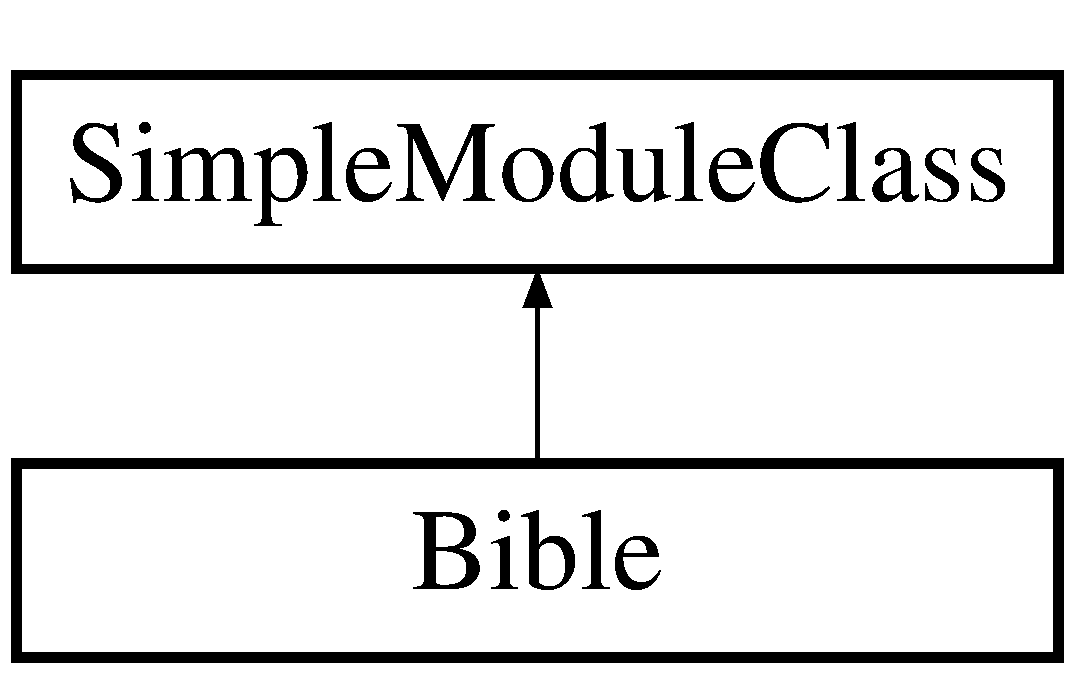
\includegraphics[height=2cm]{classBible}
\end{center}
\end{figure}
\subsection*{Public Types}
\begin{DoxyCompactItemize}
\item 
enum {\bfseries m\_\-bibleTypes} \{ {\bfseries None} =  0, 
{\bfseries BibleQuoteModule} =  1, 
{\bfseries ZefaniaBibleModule} =  2
 \}
\end{DoxyCompactItemize}
\subsection*{Public Member Functions}
\begin{DoxyCompactItemize}
\item 
\hypertarget{classBible_abbc3f50a8babc5b981463f43a526623f}{
void {\bfseries setSettings} (\hyperlink{classSettings}{Settings} $\ast$settings)}
\label{classBible_abbc3f50a8babc5b981463f43a526623f}

\item 
\hypertarget{classBible_a5d888a9ecb7988783596ba6af64b4c32}{
void {\bfseries setBibleType} (const int \&type)}
\label{classBible_a5d888a9ecb7988783596ba6af64b4c32}

\item 
\hypertarget{classBible_a755e37d040f73db48a8cb11a76cfdd9c}{
QMap$<$ int, QList$<$ \hyperlink{structChapter}{Chapter} $>$ $>$ {\bfseries getSoftCache} ()}
\label{classBible_a755e37d040f73db48a8cb11a76cfdd9c}

\item 
\hypertarget{classBible_ae5402b0e0d92d7a34a760948eebf576f}{
void {\bfseries clearSoftCache} ()}
\label{classBible_ae5402b0e0d92d7a34a760948eebf576f}

\item 
\hypertarget{classBible_a94b020a639d4f6d36766a4f3eaa3adfa}{
void {\bfseries setSoftCache} (QMap$<$ int, QList$<$ \hyperlink{structChapter}{Chapter} $>$ $>$ cache)}
\label{classBible_a94b020a639d4f6d36766a4f3eaa3adfa}

\item 
\hypertarget{classBible_afc221da9f11ff62e49588149a08eeee6}{
void {\bfseries setBibleDisplaySettings} (\hyperlink{classBibleDisplaySettings}{BibleDisplaySettings} bibleDisplaySettings)}
\label{classBible_afc221da9f11ff62e49588149a08eeee6}

\item 
\hypertarget{classBible_a6d8d6c69442ee00dab64ef12e986d22f}{
int {\bfseries loadBibleData} (const int \&bibleID, const QString \&path)}
\label{classBible_a6d8d6c69442ee00dab64ef12e986d22f}

\item 
int \hyperlink{classBible_a0057dd2ba35fe377624da860a6959cd9}{readBook} (int id)
\item 
\hypertarget{classBible_a42e0e107fa2b5966bfa90f60a0fdc3cb}{
QString {\bfseries readChapter} (int chapterID, int verseID)}
\label{classBible_a42e0e107fa2b5966bfa90f60a0fdc3cb}

\item 
QString \hyperlink{classBible_a515418999329333e8a6a821fc88d006f}{readVerse} (int chapterID, int startVerse, int endVerse, int markVerseID, bool saveRawDatas)
\item 
\hypertarget{classBible_a21a6808e0663d2f99604e137184b2b4d}{
QStringList {\bfseries getSearchPaths} ()}
\label{classBible_a21a6808e0663d2f99604e137184b2b4d}

\item 
\hypertarget{classBible_a2fe743ec79eae111c903a5b0ccfa17c9}{
QString {\bfseries toUniformHtml} (QString string)}
\label{classBible_a2fe743ec79eae111c903a5b0ccfa17c9}

\item 
\hypertarget{classBible_ab279b2e604ad7b2d445235e1302686b7}{
QStringList {\bfseries toUniformHtml} (QStringList string)}
\label{classBible_ab279b2e604ad7b2d445235e1302686b7}

\item 
\hyperlink{classSearchResult}{SearchResult} \hyperlink{classBible_a33103e25381494250b9a351572bb4e8e}{search} (\hyperlink{classSearchQuery}{SearchQuery} query)
\item 
\hypertarget{classBible_a6aeeae4c261ff3a40b28e671bed19c2d}{
int {\bfseries bibleID} ()}
\label{classBible_a6aeeae4c261ff3a40b28e671bed19c2d}

\item 
\hypertarget{classBible_a563553694b582275599e95e81ea0b3de}{
void {\bfseries setBibleID} (const int \&bible)}
\label{classBible_a563553694b582275599e95e81ea0b3de}

\item 
\hypertarget{classBible_a2df47f1e4ba133d041f458d4cf2ce6c1}{
int {\bfseries bookID} ()}
\label{classBible_a2df47f1e4ba133d041f458d4cf2ce6c1}

\item 
\hypertarget{classBible_a161d0777d83b94f31df05d32e77d76bb}{
int {\bfseries chapterID} ()}
\label{classBible_a161d0777d83b94f31df05d32e77d76bb}

\item 
\hypertarget{classBible_a7559212b56e1c9ca36f19a202c90f030}{
int {\bfseries chapterAdd} ()}
\label{classBible_a7559212b56e1c9ca36f19a202c90f030}

\item 
\hypertarget{classBible_a6c88a7a8fda28d1c6dce38d38bc7d24b}{
int {\bfseries booksCount} ()}
\label{classBible_a6c88a7a8fda28d1c6dce38d38bc7d24b}

\item 
\hypertarget{classBible_ae4b274ab0e5983243d44ae95fda1bbb6}{
int {\bfseries chaptersCount} ()}
\label{classBible_ae4b274ab0e5983243d44ae95fda1bbb6}

\end{DoxyCompactItemize}
\subsection*{Public Attributes}
\begin{DoxyCompactItemize}
\item 
\hypertarget{classBible_a61a3a3f88bdc01c6c7a493bdcbd98903}{
\hyperlink{classBibleDisplaySettings}{BibleDisplaySettings} {\bfseries m\_\-bibleDisplaySettings}}
\label{classBible_a61a3a3f88bdc01c6c7a493bdcbd98903}

\item 
\hypertarget{classBible_abced9dd0641201c2081301d2c8ff6c59}{
QString {\bfseries bibleTitle}}
\label{classBible_abced9dd0641201c2081301d2c8ff6c59}

\item 
\hypertarget{classBible_aabb92e73cdb26638d40325e5d708ec7b}{
QString {\bfseries lastout}}
\label{classBible_aabb92e73cdb26638d40325e5d708ec7b}

\item 
\hypertarget{classBible_a1287eeedb0130dcc2b9e9cea653bb4dd}{
QString {\bfseries m\_\-biblePath}}
\label{classBible_a1287eeedb0130dcc2b9e9cea653bb4dd}

\item 
\hypertarget{classBible_a1b406912e4d01a4e4755b17a6b2b3893}{
\hyperlink{classSearchQuery}{SearchQuery} {\bfseries lastSearchQuery}}
\label{classBible_a1b406912e4d01a4e4755b17a6b2b3893}

\item 
\hypertarget{classBible_a62899d799a8c6efcf5283808edb205a7}{
\hyperlink{classSearchResult}{SearchResult} {\bfseries lastSearchResult}}
\label{classBible_a62899d799a8c6efcf5283808edb205a7}

\item 
\hypertarget{classBible_ac3d84e689a0365415980d6f3ebb6e561}{
QStringList {\bfseries bookFullName}}
\label{classBible_ac3d84e689a0365415980d6f3ebb6e561}

\item 
\hypertarget{classBible_af1659c6f7db752f7c722c7880a731957}{
QStringList {\bfseries chapterText}}
\label{classBible_af1659c6f7db752f7c722c7880a731957}

\item 
\hypertarget{classBible_afcf35e16bb50b3be1d60ee74b3f8a48c}{
QStringList {\bfseries bookPath}}
\label{classBible_afcf35e16bb50b3be1d60ee74b3f8a48c}

\item 
\hypertarget{classBible_a21d4ae1646b7a8c816094bcbbec4bc88}{
QStringList {\bfseries chapterNames}}
\label{classBible_a21d4ae1646b7a8c816094bcbbec4bc88}

\item 
\hypertarget{classBible_a724de0aaf066754af1b6aa50ea554e62}{
QStringList {\bfseries chapterDataList}}
\label{classBible_a724de0aaf066754af1b6aa50ea554e62}

\item 
\hypertarget{classBible_a8ad14dd4def142176f2d04ffb213af94}{
QStringList {\bfseries biblesIniPath}}
\label{classBible_a8ad14dd4def142176f2d04ffb213af94}

\item 
\hypertarget{classBible_aed92fc6bb94809029cecfa076ae99c23}{
QMap$<$ int, int $>$ {\bfseries bookCount}}
\label{classBible_aed92fc6bb94809029cecfa076ae99c23}

\item 
\hypertarget{classBible_a1dca3a01d8a18110a1cd24337deeca80}{
QList$<$ \hyperlink{structChapter}{Chapter} $>$ {\bfseries chapterData}}
\label{classBible_a1dca3a01d8a18110a1cd24337deeca80}

\item 
\hypertarget{classBible_a2442c9bfc7b817472d62f429756ffb53}{
int {\bfseries m\_\-bibleType}}
\label{classBible_a2442c9bfc7b817472d62f429756ffb53}

\item 
\hypertarget{classBible_ab6dc84753215ebe5fc4571c5db781cb8}{
int {\bfseries m\_\-verseID}}
\label{classBible_ab6dc84753215ebe5fc4571c5db781cb8}

\item 
\hypertarget{classBible_a378fb5e8a71400bbcc14aa0bf33a6082}{
\hyperlink{classBibleQuote}{BibleQuote} {\bfseries bq}}
\label{classBible_a378fb5e8a71400bbcc14aa0bf33a6082}

\item 
\hypertarget{classBible_abae8c0e258ecb53dcf89563c7eac3fef}{
\hyperlink{classZefaniaBible}{ZefaniaBible} {\bfseries zef}}
\label{classBible_abae8c0e258ecb53dcf89563c7eac3fef}

\end{DoxyCompactItemize}


\subsection{Detailed Description}
\hyperlink{classBible}{Bible} represent a bible module(eg biblequote module)

\begin{DoxyAuthor}{Author}
Paul Walger $<$\href{mailto:metaxy@walger.name}{\tt metaxy@walger.name}$>$ 
\end{DoxyAuthor}


\subsection{Member Function Documentation}
\hypertarget{classBible_a0057dd2ba35fe377624da860a6959cd9}{
\index{Bible@{Bible}!readBook@{readBook}}
\index{readBook@{readBook}!Bible@{Bible}}
\subsubsection[{readBook}]{\setlength{\rightskip}{0pt plus 5cm}int Bible::readBook (int {\em id})}}
\label{classBible_a0057dd2ba35fe377624da860a6959cd9}
Load only the book without pharsing. \hypertarget{classBible_a515418999329333e8a6a821fc88d006f}{
\index{Bible@{Bible}!readVerse@{readVerse}}
\index{readVerse@{readVerse}!Bible@{Bible}}
\subsubsection[{readVerse}]{\setlength{\rightskip}{0pt plus 5cm}QString Bible::readVerse (int {\em chapterID}, \/  int {\em startVerse}, \/  int {\em endVerse}, \/  int {\em markVerseID} = {\ttfamily -\/1}, \/  bool {\em saveRawData} = {\ttfamily false})}}
\label{classBible_a515418999329333e8a6a821fc88d006f}
Pharse the loaded book. \hypertarget{classBible_a33103e25381494250b9a351572bb4e8e}{
\index{Bible@{Bible}!search@{search}}
\index{search@{search}!Bible@{Bible}}
\subsubsection[{search}]{\setlength{\rightskip}{0pt plus 5cm}{\bf SearchResult} Bible::search ({\bf SearchQuery} {\em query})}}
\label{classBible_a33103e25381494250b9a351572bb4e8e}
Search in the current module  The search query. 

The documentation for this class was generated from the following files:\begin{DoxyCompactItemize}
\item 
src/module/bible.h\item 
src/module/bible.cpp\end{DoxyCompactItemize}

\hypertarget{classBibleQuote}{
\section{BibleQuote Class Reference}
\label{classBibleQuote}\index{BibleQuote@{BibleQuote}}
}


{\ttfamily \#include $<$biblequote.h$>$}

\subsection*{Public Member Functions}
\begin{DoxyCompactItemize}
\item 
\hypertarget{classBibleQuote_a3d20c298cc87364e6fb9abc67352dfb9}{
int {\bfseries setSettings} (\hyperlink{classSettings}{Settings} $\ast$settings)}
\label{classBibleQuote_a3d20c298cc87364e6fb9abc67352dfb9}

\item 
\hypertarget{classBibleQuote_a42af21eb619fd89ef9bc3b6b574b0b6c}{
int {\bfseries readBook} (int id, QString path)}
\label{classBibleQuote_a42af21eb619fd89ef9bc3b6b574b0b6c}

\item 
\hypertarget{classBibleQuote_a0f9c1eb1346380d3f8e21c9cdf76390d}{
void {\bfseries loadBibleData} (int bibleID, QString path)}
\label{classBibleQuote_a0f9c1eb1346380d3f8e21c9cdf76390d}

\item 
\hypertarget{classBibleQuote_af4bd0be7d2ebf2b3fddc60757acf556a}{
QString {\bfseries readInfo} (QFile \&file)}
\label{classBibleQuote_af4bd0be7d2ebf2b3fddc60757acf556a}

\item 
\hypertarget{classBibleQuote_ab87214e63ac373631c5867e6d58cd69c}{
\hyperlink{classSearchResult}{SearchResult} {\bfseries search} (\hyperlink{classSearchQuery}{SearchQuery} query)}
\label{classBibleQuote_ab87214e63ac373631c5867e6d58cd69c}

\end{DoxyCompactItemize}
\subsection*{Public Attributes}
\begin{DoxyCompactItemize}
\item 
\hypertarget{classBibleQuote_a381b8c9746e84df1084847fc6848476b}{
int {\bfseries m\_\-bookID}}
\label{classBibleQuote_a381b8c9746e84df1084847fc6848476b}

\item 
\hypertarget{classBibleQuote_a84de51974fce2d11ef293b58996001ac}{
int {\bfseries m\_\-bibleID}}
\label{classBibleQuote_a84de51974fce2d11ef293b58996001ac}

\item 
\hypertarget{classBibleQuote_a8d7381611241b9fca7cb49fb76440950}{
bool {\bfseries chapterZero}}
\label{classBibleQuote_a8d7381611241b9fca7cb49fb76440950}

\item 
\hypertarget{classBibleQuote_affba9ada82065ed54caffe50b99d0e8c}{
QString {\bfseries currentBiblePath}}
\label{classBibleQuote_affba9ada82065ed54caffe50b99d0e8c}

\item 
\hypertarget{classBibleQuote_ac4131e3676fb7f5a1e7f935d0c576d15}{
QString {\bfseries lastout}}
\label{classBibleQuote_ac4131e3676fb7f5a1e7f935d0c576d15}

\item 
\hypertarget{classBibleQuote_a0a29f4002f140a68f2e7c8a3c27c79f1}{
QString {\bfseries chaptersign}}
\label{classBibleQuote_a0a29f4002f140a68f2e7c8a3c27c79f1}

\item 
\hypertarget{classBibleQuote_afea09fdac5376a36b46af2e51475c15e}{
QString {\bfseries versesign}}
\label{classBibleQuote_afea09fdac5376a36b46af2e51475c15e}

\item 
\hypertarget{classBibleQuote_a6269d7734c1656675a4e61be7eee31e1}{
QString {\bfseries bibleName}}
\label{classBibleQuote_a6269d7734c1656675a4e61be7eee31e1}

\item 
\hypertarget{classBibleQuote_a8ee2209de8c8b43be44216778a2e2d52}{
QString {\bfseries removeHtml}}
\label{classBibleQuote_a8ee2209de8c8b43be44216778a2e2d52}

\item 
\hypertarget{classBibleQuote_a0fd5cd1c930e285a6462831db8ca5583}{
QStringList {\bfseries bookPath}}
\label{classBibleQuote_a0fd5cd1c930e285a6462831db8ca5583}

\item 
\hypertarget{classBibleQuote_af1c9ea90b8f6dbfabe79828d4ca4e715}{
QStringList {\bfseries bookFullName}}
\label{classBibleQuote_af1c9ea90b8f6dbfabe79828d4ca4e715}

\item 
\hypertarget{classBibleQuote_af506ff787daa9c2f5342c5c13618db17}{
QStringList {\bfseries bookShortName}}
\label{classBibleQuote_af506ff787daa9c2f5342c5c13618db17}

\item 
\hypertarget{classBibleQuote_a2febae130e05447c12cd6a7cff32626f}{
QMap$<$ int, int $>$ {\bfseries bookCount}}
\label{classBibleQuote_a2febae130e05447c12cd6a7cff32626f}

\item 
\hypertarget{classBibleQuote_a8ec065ce6fa655d8dd82ba476982980c}{
\hyperlink{classSearchQuery}{SearchQuery} {\bfseries lastSearchQuery}}
\label{classBibleQuote_a8ec065ce6fa655d8dd82ba476982980c}

\item 
\hypertarget{classBibleQuote_a82725939215b4dc61f08f403c79aff61}{
QList$<$ \hyperlink{structChapter}{Chapter} $>$ {\bfseries chapterData}}
\label{classBibleQuote_a82725939215b4dc61f08f403c79aff61}

\end{DoxyCompactItemize}


\subsection{Detailed Description}
\hyperlink{classBibleQuote}{BibleQuote} represents a biblequote module

\begin{DoxyAuthor}{Author}
Paul Walger $<$\href{mailto:metaxy@walger.name}{\tt metaxy@walger.name}$>$ 
\end{DoxyAuthor}


The documentation for this class was generated from the following files:\begin{DoxyCompactItemize}
\item 
src/module/biblequote.h\item 
src/module/biblequote.cpp\end{DoxyCompactItemize}

\hypertarget{structChapter}{
\section{Chapter Struct Reference}
\label{structChapter}\index{Chapter@{Chapter}}
}


{\ttfamily \#include $<$chapter.h$>$}

\subsection*{Public Attributes}
\begin{DoxyCompactItemize}
\item 
\hypertarget{structChapter_a321e378b12d5fed1ba2fae4affdb78c7}{
QStringList {\bfseries data}}
\label{structChapter_a321e378b12d5fed1ba2fae4affdb78c7}

\item 
\hypertarget{structChapter_a29c571d490cce0129070cefe1fe0da61}{
QStringList {\bfseries verseNumber}}
\label{structChapter_a29c571d490cce0129070cefe1fe0da61}

\item 
\hypertarget{structChapter_a33e98674c40021c573e2395cc53f5dc2}{
QString {\bfseries chapterName}}
\label{structChapter_a33e98674c40021c573e2395cc53f5dc2}

\item 
\hypertarget{structChapter_a7fcbb066f25d59fb5877582ab7dad46c}{
QString {\bfseries bookName}}
\label{structChapter_a7fcbb066f25d59fb5877582ab7dad46c}

\item 
\hypertarget{structChapter_af1670eaa97d549f1d95686507665a1aa}{
int {\bfseries verseCount}}
\label{structChapter_af1670eaa97d549f1d95686507665a1aa}

\end{DoxyCompactItemize}


\subsection{Detailed Description}
\hyperlink{structChapter}{Chapter} represents a bible chapter

\begin{DoxyAuthor}{Author}
Paul Walger $<$\href{mailto:metaxy@walger.name}{\tt metaxy@walger.name}$>$ 
\end{DoxyAuthor}


The documentation for this struct was generated from the following file:\begin{DoxyCompactItemize}
\item 
src/core/chapter.h\end{DoxyCompactItemize}

\hypertarget{classDbgHelper}{
\section{DbgHelper Class Reference}
\label{classDbgHelper}\index{DbgHelper@{DbgHelper}}
}


{\ttfamily \#include $<$dbghelper.h$>$}

\subsection*{Public Member Functions}
\begin{DoxyCompactItemize}
\item 
\hypertarget{classDbgHelper_ad592120d919e04305d93c0aff04fd85f}{
{\bfseries DbgHelper} (const QString \&t)}
\label{classDbgHelper_ad592120d919e04305d93c0aff04fd85f}

\end{DoxyCompactItemize}


\subsection{Detailed Description}
\hyperlink{classDbgHelper}{DbgHelper} is a debug helper, it show the debug ouput more clearly

\begin{DoxyAuthor}{Author}
Paul Walger $<$\href{mailto:metaxy@walger.name}{\tt metaxy@walger.name}$>$ 
\end{DoxyAuthor}


The documentation for this class was generated from the following files:\begin{DoxyCompactItemize}
\item 
src/core/dbghelper.h\item 
src/core/dbghelper.cpp\end{DoxyCompactItemize}

\hypertarget{classGoTo}{
\section{GoTo Class Reference}
\label{classGoTo}\index{GoTo@{GoTo}}
}


{\ttfamily \#include $<$goto.h$>$}\subsection*{Public Member Functions}
\begin{DoxyCompactItemize}
\item 
\hypertarget{classGoTo_af65860fd8cbfde047a2ac0b848c08ccb}{
{\bfseries GoTo} (int currentBibleID, QStringList bookFullName)}
\label{classGoTo_af65860fd8cbfde047a2ac0b848c08ccb}

\item 
\hypertarget{classGoTo_abeb80d20c63ea781fb6426690b11a8c1}{
QString {\bfseries getUrl} (const QString \&text)}
\label{classGoTo_abeb80d20c63ea781fb6426690b11a8c1}

\end{DoxyCompactItemize}


\subsection{Detailed Description}
\hyperlink{classGoTo}{GoTo} is a pharser for bible passage into a url

\begin{DoxyAuthor}{Author}
Paul Walger $<$\href{mailto:metaxy@walger.name}{\tt metaxy@walger.name}$>$ 
\end{DoxyAuthor}


The documentation for this class was generated from the following files:\begin{DoxyCompactItemize}
\item 
src/core/goto.h\item 
src/core/goto.cpp\end{DoxyCompactItemize}

\hypertarget{classHistory}{
\section{History Class Reference}
\label{classHistory}\index{History@{History}}
}
{\tt \#include $<$history.h$>$}

\subsection*{Public Member Functions}
\begin{CompactItemize}
\item 
QString \hyperlink{classHistory_83d69c4bfe79d19a6187f586e7311b22}{forward} ()
\item 
QString \hyperlink{classHistory_41c8d23cb2789b07bc6229b203bafce3}{backward} ()
\item 
bool \hyperlink{classHistory_1227493ba04f3f640c6648b9562bf68e}{forwardAvailable} ()
\item 
bool \hyperlink{classHistory_c8c3f249e76605c9686eacb4716c79b4}{backwardAvailable} ()
\item 
void \hyperlink{classHistory_7fd72e5b7289c61f32ec5d533d0356bf}{setCurrent} (const QString \&current)
\end{CompactItemize}


\subsection{Detailed Description}
\hyperlink{classHistory}{History} is a simple class to get a url history

\begin{Desc}
\item[Author:]Paul Walger $<$\href{mailto:metaxy@walger.name}{\tt metaxy@walger.name}$>$ \end{Desc}


\subsection{Member Function Documentation}
\hypertarget{classHistory_41c8d23cb2789b07bc6229b203bafce3}{
\index{History@{History}!backward@{backward}}
\index{backward@{backward}!History@{History}}
\subsubsection[{backward}]{\setlength{\rightskip}{0pt plus 5cm}QString History::backward ()}}
\label{classHistory_41c8d23cb2789b07bc6229b203bafce3}


Return the previous url in the history. \hypertarget{classHistory_c8c3f249e76605c9686eacb4716c79b4}{
\index{History@{History}!backwardAvailable@{backwardAvailable}}
\index{backwardAvailable@{backwardAvailable}!History@{History}}
\subsubsection[{backwardAvailable}]{\setlength{\rightskip}{0pt plus 5cm}bool History::backwardAvailable ()}}
\label{classHistory_c8c3f249e76605c9686eacb4716c79b4}


Check if a prevoius url is available. \hypertarget{classHistory_83d69c4bfe79d19a6187f586e7311b22}{
\index{History@{History}!forward@{forward}}
\index{forward@{forward}!History@{History}}
\subsubsection[{forward}]{\setlength{\rightskip}{0pt plus 5cm}QString History::forward ()}}
\label{classHistory_83d69c4bfe79d19a6187f586e7311b22}


Return the next url in the history. \hypertarget{classHistory_1227493ba04f3f640c6648b9562bf68e}{
\index{History@{History}!forwardAvailable@{forwardAvailable}}
\index{forwardAvailable@{forwardAvailable}!History@{History}}
\subsubsection[{forwardAvailable}]{\setlength{\rightskip}{0pt plus 5cm}bool History::forwardAvailable ()}}
\label{classHistory_1227493ba04f3f640c6648b9562bf68e}


Check if a next url is available. \hypertarget{classHistory_7fd72e5b7289c61f32ec5d533d0356bf}{
\index{History@{History}!setCurrent@{setCurrent}}
\index{setCurrent@{setCurrent}!History@{History}}
\subsubsection[{setCurrent}]{\setlength{\rightskip}{0pt plus 5cm}void History::setCurrent (const QString \& {\em url})}}
\label{classHistory_7fd72e5b7289c61f32ec5d533d0356bf}


Add a new url to the history. \begin{Desc}
\item[Parameters:]
\begin{description}
\item[{\em url}]the new url \end{description}
\end{Desc}


The documentation for this class was generated from the following files:\begin{CompactItemize}
\item 
src/core/history.h\item 
src/core/history.cpp\end{CompactItemize}

\hypertarget{classKoXmlCDATASection}{
\section{KoXmlCDATASection Class Reference}
\label{classKoXmlCDATASection}\index{KoXmlCDATASection@{KoXmlCDATASection}}
}


{\ttfamily \#include $<$KoXmlReader.h$>$}Inheritance diagram for KoXmlCDATASection::\begin{figure}[H]
\begin{center}
\leavevmode
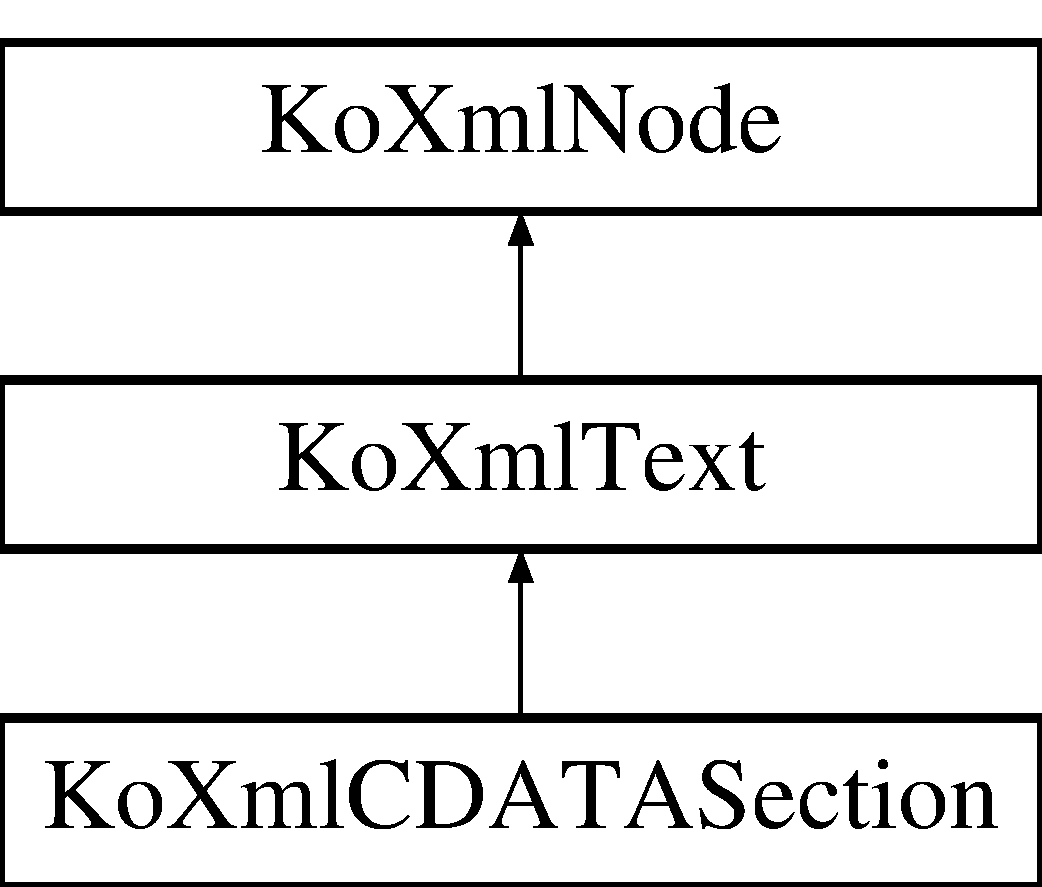
\includegraphics[height=3cm]{classKoXmlCDATASection}
\end{center}
\end{figure}
\subsection*{Public Member Functions}
\begin{DoxyCompactItemize}
\item 
\hypertarget{classKoXmlCDATASection_a9f69382bc27884731599f49763926343}{
{\bfseries KoXmlCDATASection} (const \hyperlink{classKoXmlCDATASection}{KoXmlCDATASection} \&cdata)}
\label{classKoXmlCDATASection_a9f69382bc27884731599f49763926343}

\item 
\hypertarget{classKoXmlCDATASection_a2380c3e02c07e9f31ee30c97de202c06}{
\hyperlink{classKoXmlCDATASection}{KoXmlCDATASection} \& {\bfseries operator=} (const \hyperlink{classKoXmlCDATASection}{KoXmlCDATASection} \&cdata)}
\label{classKoXmlCDATASection_a2380c3e02c07e9f31ee30c97de202c06}

\item 
\hypertarget{classKoXmlCDATASection_af5d118d633fa233c8a7c9a3fad7ae5fd}{
virtual bool {\bfseries isCDATASection} () const }
\label{classKoXmlCDATASection_af5d118d633fa233c8a7c9a3fad7ae5fd}

\end{DoxyCompactItemize}
\subsection*{Friends}
\begin{DoxyCompactItemize}
\item 
\hypertarget{classKoXmlCDATASection_a6c97883f92c7cbf2ecdf17db6cea8297}{
class \hyperlink{classKoXmlCDATASection_a6c97883f92c7cbf2ecdf17db6cea8297}{KoXmlNode}}
\label{classKoXmlCDATASection_a6c97883f92c7cbf2ecdf17db6cea8297}

\item 
\hypertarget{classKoXmlCDATASection_a7f0a67ef52ddc6542737225a82e4f487}{
class \hyperlink{classKoXmlCDATASection_a7f0a67ef52ddc6542737225a82e4f487}{KoXmlDocument}}
\label{classKoXmlCDATASection_a7f0a67ef52ddc6542737225a82e4f487}

\end{DoxyCompactItemize}


\subsection{Detailed Description}
\hyperlink{classKoXmlCDATASection}{KoXmlCDATASection} represents a CDATA section in a DOM tree. \begin{DoxyAuthor}{Author}
Ariya Hidayat $<$\href{mailto:ariya@kde.org}{\tt ariya@kde.org}$>$ 
\end{DoxyAuthor}


The documentation for this class was generated from the following files:\begin{DoxyCompactItemize}
\item 
src/core/KoXmlReader.h\item 
src/core/KoXmlReader.cpp\end{DoxyCompactItemize}

\hypertarget{classKoXmlDocument}{
\section{KoXmlDocument Class Reference}
\label{classKoXmlDocument}\index{KoXmlDocument@{KoXmlDocument}}
}


{\ttfamily \#include $<$KoXmlReader.h$>$}

Inheritance diagram for KoXmlDocument:\begin{figure}[H]
\begin{center}
\leavevmode
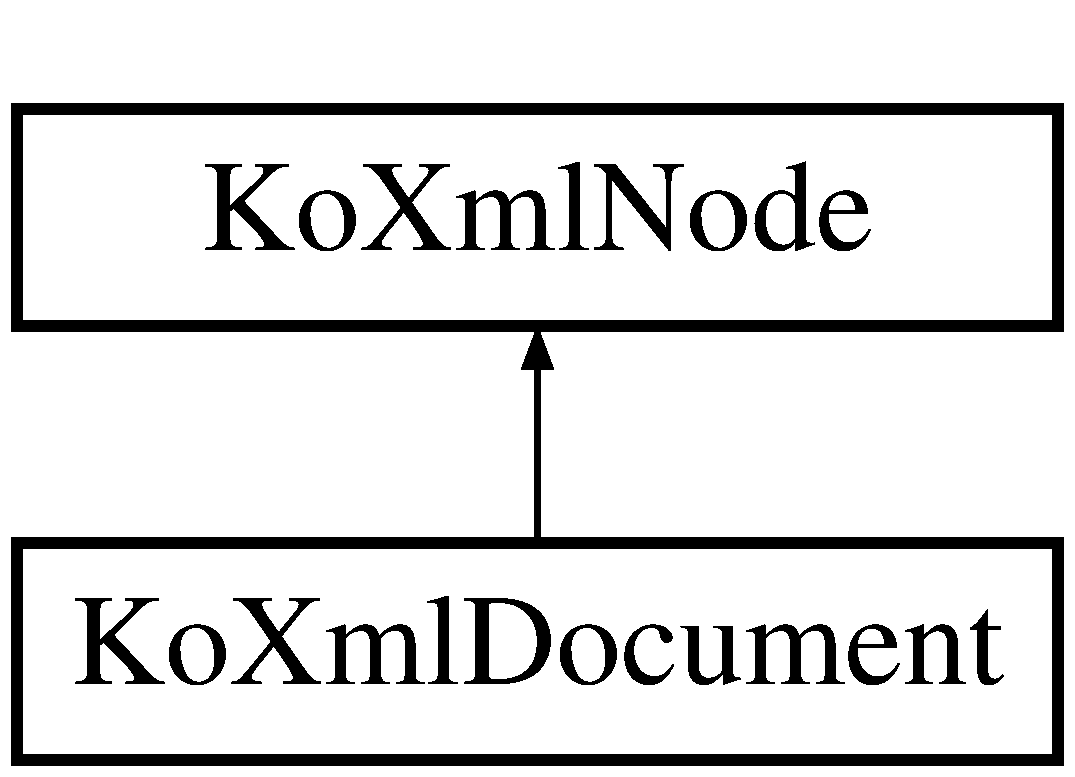
\includegraphics[height=2cm]{classKoXmlDocument}
\end{center}
\end{figure}
\subsection*{Public Member Functions}
\begin{DoxyCompactItemize}
\item 
\hypertarget{classKoXmlDocument_a25098f08f373e4b0ac8115279eb65c8b}{
{\bfseries KoXmlDocument} (const \hyperlink{classKoXmlDocument}{KoXmlDocument} \&node)}
\label{classKoXmlDocument_a25098f08f373e4b0ac8115279eb65c8b}

\item 
\hypertarget{classKoXmlDocument_aae3cf314dc2212a6930689a565e9b674}{
\hyperlink{classKoXmlDocument}{KoXmlDocument} \& {\bfseries operator=} (const \hyperlink{classKoXmlDocument}{KoXmlDocument} \&node)}
\label{classKoXmlDocument_aae3cf314dc2212a6930689a565e9b674}

\item 
\hypertarget{classKoXmlDocument_a94a468069c36d6bb136fe5aa0cf850f1}{
bool {\bfseries operator==} (const \hyperlink{classKoXmlDocument}{KoXmlDocument} \&) const }
\label{classKoXmlDocument_a94a468069c36d6bb136fe5aa0cf850f1}

\item 
\hypertarget{classKoXmlDocument_a4f791e9965cdf7098c7aa50e40b0bb43}{
bool {\bfseries operator!=} (const \hyperlink{classKoXmlDocument}{KoXmlDocument} \&) const }
\label{classKoXmlDocument_a4f791e9965cdf7098c7aa50e40b0bb43}

\item 
\hypertarget{classKoXmlDocument_a1f15d923c78de93d044de05097f9bdcb}{
\hyperlink{classKoXmlElement}{KoXmlElement} {\bfseries documentElement} () const }
\label{classKoXmlDocument_a1f15d923c78de93d044de05097f9bdcb}

\item 
\hypertarget{classKoXmlDocument_a6266b024d223083496a47251012787c2}{
\hyperlink{classKoXmlDocumentType}{KoXmlDocumentType} {\bfseries doctype} () const }
\label{classKoXmlDocument_a6266b024d223083496a47251012787c2}

\item 
\hypertarget{classKoXmlDocument_a8e6196e9bfc792164d8c481bb7f11fcd}{
virtual QString {\bfseries nodeName} () const }
\label{classKoXmlDocument_a8e6196e9bfc792164d8c481bb7f11fcd}

\item 
\hypertarget{classKoXmlDocument_a5291c35721c45c0109176d9db6162fee}{
virtual void {\bfseries clear} ()}
\label{classKoXmlDocument_a5291c35721c45c0109176d9db6162fee}

\item 
\hypertarget{classKoXmlDocument_ae9f84dc9b1ae3cd561628fbcb4b0d0e5}{
bool {\bfseries setContent} (QIODevice $\ast$device, bool namespaceProcessing, QString $\ast$errorMsg=0, int $\ast$errorLine=0, int $\ast$errorColumn=0)}
\label{classKoXmlDocument_ae9f84dc9b1ae3cd561628fbcb4b0d0e5}

\item 
\hypertarget{classKoXmlDocument_ae14a8ad6b1c2d80acd8416900c1e04d7}{
bool {\bfseries setContent} (QIODevice $\ast$device, QString $\ast$errorMsg=0, int $\ast$errorLine=0, int $\ast$errorColumn=0)}
\label{classKoXmlDocument_ae14a8ad6b1c2d80acd8416900c1e04d7}

\item 
\hypertarget{classKoXmlDocument_a9985cf50d73165c1de6140d1bcec48ff}{
bool {\bfseries setContent} (QXmlInputSource $\ast$source, QXmlReader $\ast$reader, QString $\ast$errorMsg=0, int $\ast$errorLine=0, int $\ast$errorColumn=0)}
\label{classKoXmlDocument_a9985cf50d73165c1de6140d1bcec48ff}

\item 
\hypertarget{classKoXmlDocument_a95a6f5727a5b9b494c3c6cf071b41c9c}{
bool {\bfseries setContent} (const QByteArray \&text, bool namespaceProcessing, QString $\ast$errorMsg=0, int $\ast$errorLine=0, int $\ast$errorColumn=0)}
\label{classKoXmlDocument_a95a6f5727a5b9b494c3c6cf071b41c9c}

\item 
\hypertarget{classKoXmlDocument_a1a35de2b10068b15f7db3f35a9e78768}{
bool {\bfseries setContent} (const QString \&text, bool namespaceProcessing, QString $\ast$errorMsg=0, int $\ast$errorLine=0, int $\ast$errorColumn=0)}
\label{classKoXmlDocument_a1a35de2b10068b15f7db3f35a9e78768}

\item 
\hypertarget{classKoXmlDocument_a45df03a6aac81990c5ad19975126f5b3}{
bool {\bfseries setContent} (const QString \&text, QString $\ast$errorMsg=0, int $\ast$errorLine=0, int $\ast$errorColumn=0)}
\label{classKoXmlDocument_a45df03a6aac81990c5ad19975126f5b3}

\end{DoxyCompactItemize}
\subsection*{Friends}
\begin{DoxyCompactItemize}
\item 
\hypertarget{classKoXmlDocument_a6c97883f92c7cbf2ecdf17db6cea8297}{
class \hyperlink{classKoXmlDocument_a6c97883f92c7cbf2ecdf17db6cea8297}{KoXmlNode}}
\label{classKoXmlDocument_a6c97883f92c7cbf2ecdf17db6cea8297}

\end{DoxyCompactItemize}


\subsection{Detailed Description}
\hyperlink{classKoXmlDocument}{KoXmlDocument} represents an XML document, structured in a DOM tree.

\hyperlink{classKoXmlDocument}{KoXmlDocument} is designed to be memory efficient. Unlike QDomDocument from Qt's XML module, \hyperlink{classKoXmlDocument}{KoXmlDocument} does not store all nodes in the DOM tree. Some nodes will be loaded and parsed on-\/demand only.

\hyperlink{classKoXmlDocument}{KoXmlDocument} is read-\/only, you can not modify its content.

\begin{DoxyAuthor}{Author}
Ariya Hidayat $<$\href{mailto:ariya@kde.org}{\tt ariya@kde.org}$>$ 
\end{DoxyAuthor}


The documentation for this class was generated from the following files:\begin{DoxyCompactItemize}
\item 
src/core/KoXmlReader.h\item 
src/core/KoXmlReader.cpp\end{DoxyCompactItemize}

\hypertarget{classKoXmlDocumentType}{
\section{KoXmlDocumentType Class Reference}
\label{classKoXmlDocumentType}\index{KoXmlDocumentType@{KoXmlDocumentType}}
}


{\ttfamily \#include $<$KoXmlReader.h$>$}Inheritance diagram for KoXmlDocumentType::\begin{figure}[H]
\begin{center}
\leavevmode
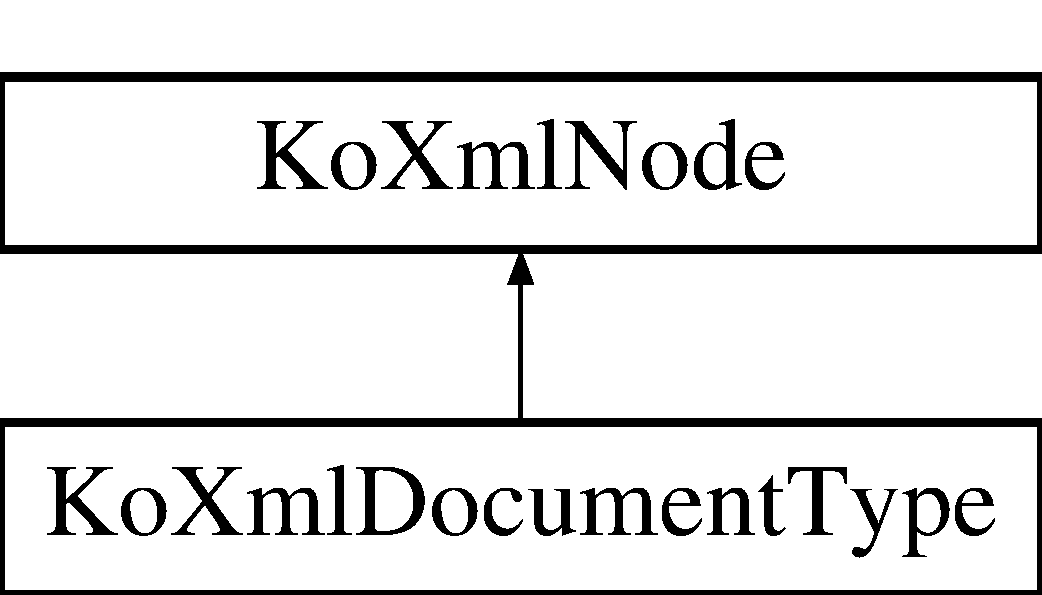
\includegraphics[height=2cm]{classKoXmlDocumentType}
\end{center}
\end{figure}
\subsection*{Public Member Functions}
\begin{DoxyCompactItemize}
\item 
\hypertarget{classKoXmlDocumentType_a8fab4dbc84e6de8408ae05043525740a}{
{\bfseries KoXmlDocumentType} (const \hyperlink{classKoXmlDocumentType}{KoXmlDocumentType} \&)}
\label{classKoXmlDocumentType_a8fab4dbc84e6de8408ae05043525740a}

\item 
\hypertarget{classKoXmlDocumentType_ab013c4a30060086de2797764414ca95c}{
\hyperlink{classKoXmlDocumentType}{KoXmlDocumentType} \& {\bfseries operator=} (const \hyperlink{classKoXmlDocumentType}{KoXmlDocumentType} \&)}
\label{classKoXmlDocumentType_ab013c4a30060086de2797764414ca95c}

\item 
\hypertarget{classKoXmlDocumentType_aa383d3090676752ae75bf24325a44003}{
QString {\bfseries name} () const }
\label{classKoXmlDocumentType_aa383d3090676752ae75bf24325a44003}

\end{DoxyCompactItemize}
\subsection*{Friends}
\begin{DoxyCompactItemize}
\item 
\hypertarget{classKoXmlDocumentType_a6c97883f92c7cbf2ecdf17db6cea8297}{
class \hyperlink{classKoXmlDocumentType_a6c97883f92c7cbf2ecdf17db6cea8297}{KoXmlNode}}
\label{classKoXmlDocumentType_a6c97883f92c7cbf2ecdf17db6cea8297}

\item 
\hypertarget{classKoXmlDocumentType_a7f0a67ef52ddc6542737225a82e4f487}{
class \hyperlink{classKoXmlDocumentType_a7f0a67ef52ddc6542737225a82e4f487}{KoXmlDocument}}
\label{classKoXmlDocumentType_a7f0a67ef52ddc6542737225a82e4f487}

\end{DoxyCompactItemize}


\subsection{Detailed Description}
\hyperlink{classKoXmlDocumentType}{KoXmlDocumentType} represents the DTD of the document. At the moment, it can used only to get the document type, i.e. no support for entities etc.

\begin{DoxyAuthor}{Author}
Ariya Hidayat $<$\href{mailto:ariya@kde.org}{\tt ariya@kde.org}$>$ 
\end{DoxyAuthor}


The documentation for this class was generated from the following files:\begin{DoxyCompactItemize}
\item 
src/core/KoXmlReader.h\item 
src/core/KoXmlReader.cpp\end{DoxyCompactItemize}

\hypertarget{classKoXmlElement}{
\section{KoXmlElement Class Reference}
\label{classKoXmlElement}\index{KoXmlElement@{KoXmlElement}}
}


{\ttfamily \#include $<$KoXmlReader.h$>$}Inheritance diagram for KoXmlElement::\begin{figure}[H]
\begin{center}
\leavevmode
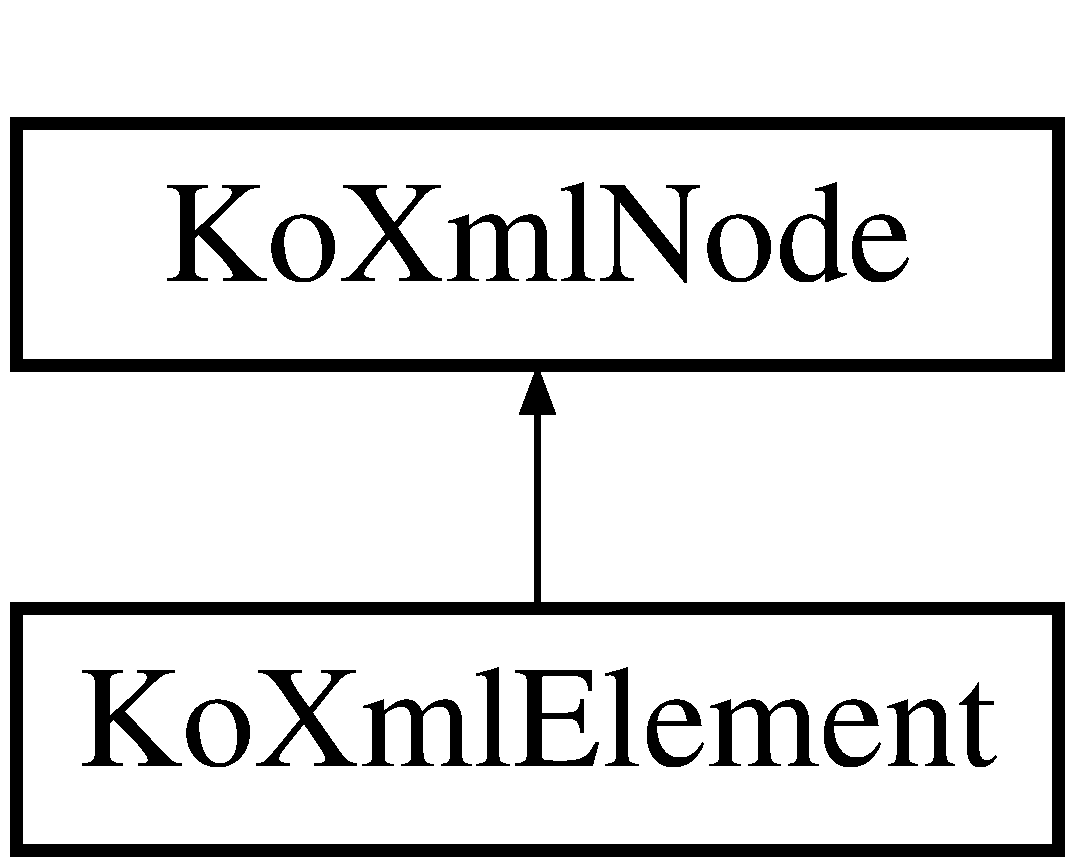
\includegraphics[height=2cm]{classKoXmlElement}
\end{center}
\end{figure}
\subsection*{Public Member Functions}
\begin{DoxyCompactItemize}
\item 
\hypertarget{classKoXmlElement_ab5637448b6070d8ac7a84ab56890ca10}{
{\bfseries KoXmlElement} (const \hyperlink{classKoXmlElement}{KoXmlElement} \&element)}
\label{classKoXmlElement_ab5637448b6070d8ac7a84ab56890ca10}

\item 
\hypertarget{classKoXmlElement_aeadd8e4eb16e9e3e3b9d2920fd183a34}{
\hyperlink{classKoXmlElement}{KoXmlElement} \& {\bfseries operator=} (const \hyperlink{classKoXmlElement}{KoXmlElement} \&element)}
\label{classKoXmlElement_aeadd8e4eb16e9e3e3b9d2920fd183a34}

\item 
\hypertarget{classKoXmlElement_a83343b34a11ddcbe2bb896a37ea41b1a}{
bool {\bfseries operator==} (const \hyperlink{classKoXmlElement}{KoXmlElement} \&) const }
\label{classKoXmlElement_a83343b34a11ddcbe2bb896a37ea41b1a}

\item 
\hypertarget{classKoXmlElement_a85276f0c883f6af251d52548dcb2e01f}{
bool {\bfseries operator!=} (const \hyperlink{classKoXmlElement}{KoXmlElement} \&) const }
\label{classKoXmlElement_a85276f0c883f6af251d52548dcb2e01f}

\item 
\hypertarget{classKoXmlElement_a5a89263ce785d65bce2bd068fc2bcb54}{
QString {\bfseries tagName} () const }
\label{classKoXmlElement_a5a89263ce785d65bce2bd068fc2bcb54}

\item 
\hypertarget{classKoXmlElement_a88971f674463f29dc7c5ac8923b75cd7}{
QString {\bfseries text} () const }
\label{classKoXmlElement_a88971f674463f29dc7c5ac8923b75cd7}

\item 
\hypertarget{classKoXmlElement_a155d0ddfa0e45922fb485dc686da1b66}{
QString {\bfseries attribute} (const QString \&name) const }
\label{classKoXmlElement_a155d0ddfa0e45922fb485dc686da1b66}

\item 
\hypertarget{classKoXmlElement_a0bd29a6227d6e8d9863734f5a3ed7fbd}{
QString {\bfseries attribute} (const QString \&name, const QString \&defaultValue) const }
\label{classKoXmlElement_a0bd29a6227d6e8d9863734f5a3ed7fbd}

\item 
\hypertarget{classKoXmlElement_ada688c66b5cd1cecf0711de63fe8f347}{
QString {\bfseries attributeNS} (const QString \&namespaceURI, const QString \&localName, const QString \&defaultValue=QString()) const }
\label{classKoXmlElement_ada688c66b5cd1cecf0711de63fe8f347}

\item 
\hypertarget{classKoXmlElement_a2a4784923c11d9d33ce187b55c562601}{
bool {\bfseries hasAttribute} (const QString \&name) const }
\label{classKoXmlElement_a2a4784923c11d9d33ce187b55c562601}

\item 
\hypertarget{classKoXmlElement_a8879ebfc276ad89f9de6aa3dab5b063d}{
bool {\bfseries hasAttributeNS} (const QString \&namespaceURI, const QString \&localName) const }
\label{classKoXmlElement_a8879ebfc276ad89f9de6aa3dab5b063d}

\end{DoxyCompactItemize}
\subsection*{Friends}
\begin{DoxyCompactItemize}
\item 
\hypertarget{classKoXmlElement_a6c97883f92c7cbf2ecdf17db6cea8297}{
class \hyperlink{classKoXmlElement_a6c97883f92c7cbf2ecdf17db6cea8297}{KoXmlNode}}
\label{classKoXmlElement_a6c97883f92c7cbf2ecdf17db6cea8297}

\item 
\hypertarget{classKoXmlElement_a7f0a67ef52ddc6542737225a82e4f487}{
class \hyperlink{classKoXmlElement_a7f0a67ef52ddc6542737225a82e4f487}{KoXmlDocument}}
\label{classKoXmlElement_a7f0a67ef52ddc6542737225a82e4f487}

\end{DoxyCompactItemize}


\subsection{Detailed Description}
\hyperlink{classKoXmlElement}{KoXmlElement} represents a tag element in a DOM tree.

\hyperlink{classKoXmlElement}{KoXmlElement} holds information about an XML tag, along with its attributes.

\begin{DoxyAuthor}{Author}
Ariya Hidayat $<$\href{mailto:ariya@kde.org}{\tt ariya@kde.org}$>$ 
\end{DoxyAuthor}


The documentation for this class was generated from the following files:\begin{DoxyCompactItemize}
\item 
src/core/KoXmlReader.h\item 
src/core/KoXmlReader.cpp\end{DoxyCompactItemize}

\hypertarget{classKoXmlNode}{
\section{KoXmlNode Class Reference}
\label{classKoXmlNode}\index{KoXmlNode@{KoXmlNode}}
}


{\ttfamily \#include $<$KoXmlReader.h$>$}Inheritance diagram for KoXmlNode::\begin{figure}[H]
\begin{center}
\leavevmode
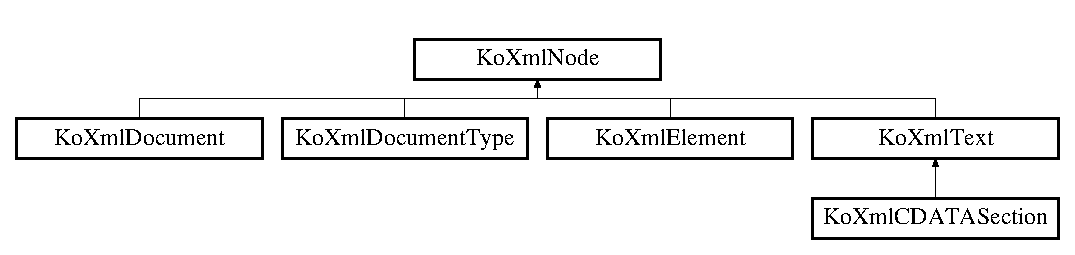
\includegraphics[height=2.97872cm]{classKoXmlNode}
\end{center}
\end{figure}
\subsection*{Public Types}
\begin{DoxyCompactItemize}
\item 
enum {\bfseries NodeType} \{ \par
{\bfseries NullNode} =  0, 
{\bfseries ElementNode}, 
{\bfseries TextNode}, 
{\bfseries CDATASectionNode}, 
\par
{\bfseries ProcessingInstructionNode}, 
{\bfseries DocumentNode}, 
{\bfseries DocumentTypeNode}
 \}
\end{DoxyCompactItemize}
\subsection*{Public Member Functions}
\begin{DoxyCompactItemize}
\item 
\hypertarget{classKoXmlNode_ab88c9ac0386a4c92ede215f97afc87e3}{
{\bfseries KoXmlNode} (const \hyperlink{classKoXmlNode}{KoXmlNode} \&node)}
\label{classKoXmlNode_ab88c9ac0386a4c92ede215f97afc87e3}

\item 
\hypertarget{classKoXmlNode_a06a42651d8b1d8d46ccfd963789d28a3}{
\hyperlink{classKoXmlNode}{KoXmlNode} \& {\bfseries operator=} (const \hyperlink{classKoXmlNode}{KoXmlNode} \&node)}
\label{classKoXmlNode_a06a42651d8b1d8d46ccfd963789d28a3}

\item 
\hypertarget{classKoXmlNode_a0c491bd3aa1f60c7c2f8aa66fcaf7ad4}{
bool {\bfseries operator==} (const \hyperlink{classKoXmlNode}{KoXmlNode} \&) const }
\label{classKoXmlNode_a0c491bd3aa1f60c7c2f8aa66fcaf7ad4}

\item 
\hypertarget{classKoXmlNode_aa7320ffe46fab32645e9f912793318df}{
bool {\bfseries operator!=} (const \hyperlink{classKoXmlNode}{KoXmlNode} \&) const }
\label{classKoXmlNode_aa7320ffe46fab32645e9f912793318df}

\item 
\hypertarget{classKoXmlNode_a8fdc94c286b2ee40ed1d3e418739245a}{
virtual KoXmlNode::NodeType {\bfseries nodeType} () const }
\label{classKoXmlNode_a8fdc94c286b2ee40ed1d3e418739245a}

\item 
\hypertarget{classKoXmlNode_a93fadc49d9739def1d0377760b804294}{
virtual bool {\bfseries isNull} () const }
\label{classKoXmlNode_a93fadc49d9739def1d0377760b804294}

\item 
\hypertarget{classKoXmlNode_a27d714ac8a277c16d90cbeaf87e23105}{
virtual bool {\bfseries isElement} () const }
\label{classKoXmlNode_a27d714ac8a277c16d90cbeaf87e23105}

\item 
\hypertarget{classKoXmlNode_a1018dd29ae7b00e453bd577764b71ecd}{
virtual bool {\bfseries isText} () const }
\label{classKoXmlNode_a1018dd29ae7b00e453bd577764b71ecd}

\item 
\hypertarget{classKoXmlNode_ae84ca4ef65b1d85ed8b90a07fb324fc8}{
virtual bool {\bfseries isCDATASection} () const }
\label{classKoXmlNode_ae84ca4ef65b1d85ed8b90a07fb324fc8}

\item 
\hypertarget{classKoXmlNode_a72089a94f37917bdc8896368c83c75dd}{
virtual bool {\bfseries isDocument} () const }
\label{classKoXmlNode_a72089a94f37917bdc8896368c83c75dd}

\item 
\hypertarget{classKoXmlNode_ac959bde05fba69bc9593e45e8862e7fd}{
virtual bool {\bfseries isDocumentType} () const }
\label{classKoXmlNode_ac959bde05fba69bc9593e45e8862e7fd}

\item 
\hypertarget{classKoXmlNode_a514c6e4cca00c3cdd15b49b7256ccdca}{
virtual void {\bfseries clear} ()}
\label{classKoXmlNode_a514c6e4cca00c3cdd15b49b7256ccdca}

\item 
\hypertarget{classKoXmlNode_af4ecc91ee34dc96cce56baf014f33618}{
\hyperlink{classKoXmlElement}{KoXmlElement} {\bfseries toElement} () const }
\label{classKoXmlNode_af4ecc91ee34dc96cce56baf014f33618}

\item 
\hypertarget{classKoXmlNode_a0a59d93ef6d9470fd45eb4b9e9c36ef1}{
\hyperlink{classKoXmlText}{KoXmlText} {\bfseries toText} () const }
\label{classKoXmlNode_a0a59d93ef6d9470fd45eb4b9e9c36ef1}

\item 
\hypertarget{classKoXmlNode_ab78d1e67e9ebda2ea669e66d28e855d9}{
\hyperlink{classKoXmlCDATASection}{KoXmlCDATASection} {\bfseries toCDATASection} () const }
\label{classKoXmlNode_ab78d1e67e9ebda2ea669e66d28e855d9}

\item 
\hypertarget{classKoXmlNode_aa0abff287194be42fb8a481c00c0e9e6}{
\hyperlink{classKoXmlDocument}{KoXmlDocument} {\bfseries toDocument} () const }
\label{classKoXmlNode_aa0abff287194be42fb8a481c00c0e9e6}

\item 
\hypertarget{classKoXmlNode_aa20285fa94dca94fddc354564d0c88be}{
virtual QString {\bfseries nodeName} () const }
\label{classKoXmlNode_aa20285fa94dca94fddc354564d0c88be}

\item 
\hypertarget{classKoXmlNode_acb26ec1c77974dfa349e56f371ec21c5}{
virtual QString {\bfseries namespaceURI} () const }
\label{classKoXmlNode_acb26ec1c77974dfa349e56f371ec21c5}

\item 
\hypertarget{classKoXmlNode_a204cfe128f5b60d2f138e1733f457402}{
virtual QString {\bfseries prefix} () const }
\label{classKoXmlNode_a204cfe128f5b60d2f138e1733f457402}

\item 
\hypertarget{classKoXmlNode_a12a19b317412059a47df882f6e66c6af}{
virtual QString {\bfseries localName} () const }
\label{classKoXmlNode_a12a19b317412059a47df882f6e66c6af}

\item 
\hypertarget{classKoXmlNode_a5e7fa60afab968f744a5424da70699e4}{
\hyperlink{classKoXmlDocument}{KoXmlDocument} {\bfseries ownerDocument} () const }
\label{classKoXmlNode_a5e7fa60afab968f744a5424da70699e4}

\item 
\hypertarget{classKoXmlNode_a50fb2d47e886a098fb369009939d08ad}{
\hyperlink{classKoXmlNode}{KoXmlNode} {\bfseries parentNode} () const }
\label{classKoXmlNode_a50fb2d47e886a098fb369009939d08ad}

\item 
\hypertarget{classKoXmlNode_acaa00c62da8540db16ecbd54b953a1fc}{
bool {\bfseries hasChildNodes} () const }
\label{classKoXmlNode_acaa00c62da8540db16ecbd54b953a1fc}

\item 
\hypertarget{classKoXmlNode_a144685aade56a4ba964452de8fa6e6e4}{
\hyperlink{classKoXmlNode}{KoXmlNode} {\bfseries firstChild} () const }
\label{classKoXmlNode_a144685aade56a4ba964452de8fa6e6e4}

\item 
\hypertarget{classKoXmlNode_aea16e2bca4f13dc87872a6f5a39647b7}{
\hyperlink{classKoXmlNode}{KoXmlNode} {\bfseries lastChild} () const }
\label{classKoXmlNode_aea16e2bca4f13dc87872a6f5a39647b7}

\item 
\hypertarget{classKoXmlNode_a422d7bd0d5107a2e062a22ddccf0220a}{
\hyperlink{classKoXmlNode}{KoXmlNode} {\bfseries nextSibling} () const }
\label{classKoXmlNode_a422d7bd0d5107a2e062a22ddccf0220a}

\item 
\hypertarget{classKoXmlNode_a48e2e9b58a3a67307e6950476cb6dde5}{
\hyperlink{classKoXmlNode}{KoXmlNode} {\bfseries previousSibling} () const }
\label{classKoXmlNode_a48e2e9b58a3a67307e6950476cb6dde5}

\item 
\hypertarget{classKoXmlNode_afa7807761c17f1c4c49fae6d4702a3c6}{
int {\bfseries childNodesCount} () const }
\label{classKoXmlNode_afa7807761c17f1c4c49fae6d4702a3c6}

\item 
\hypertarget{classKoXmlNode_a4cbefc4c323ee9b422b568a141463feb}{
QStringList {\bfseries attributeNames} () const }
\label{classKoXmlNode_a4cbefc4c323ee9b422b568a141463feb}

\item 
\hypertarget{classKoXmlNode_a3c1e84615051a447ad66de67b4cb3b51}{
\hyperlink{classKoXmlNode}{KoXmlNode} {\bfseries namedItem} (const QString \&name) const }
\label{classKoXmlNode_a3c1e84615051a447ad66de67b4cb3b51}

\item 
\hypertarget{classKoXmlNode_a875cc1bd632bdce741ef0e64c2e8e348}{
\hyperlink{classKoXmlNode}{KoXmlNode} {\bfseries namedItemNS} (const QString \&nsURI, const QString \&name) const }
\label{classKoXmlNode_a875cc1bd632bdce741ef0e64c2e8e348}

\item 
void \hyperlink{classKoXmlNode_a00f067df3c054abdb722f3cdf372f58f}{load} (int depth=1)
\item 
void \hyperlink{classKoXmlNode_a6db615544f532dec26530d2fe413c946}{unload} ()
\item 
\hypertarget{classKoXmlNode_acc8aa6574d8389e8ba9e1bc758d1038d}{
QDomNode {\bfseries asQDomNode} (QDomDocument ownerDoc) const }
\label{classKoXmlNode_acc8aa6574d8389e8ba9e1bc758d1038d}

\end{DoxyCompactItemize}
\subsection*{Protected Member Functions}
\begin{DoxyCompactItemize}
\item 
\hypertarget{classKoXmlNode_a150c3bcb9ccb9978784733a72fc56230}{
{\bfseries KoXmlNode} (\hyperlink{classKoXmlNodeData}{KoXmlNodeData} $\ast$)}
\label{classKoXmlNode_a150c3bcb9ccb9978784733a72fc56230}

\end{DoxyCompactItemize}
\subsection*{Protected Attributes}
\begin{DoxyCompactItemize}
\item 
\hypertarget{classKoXmlNode_a09a35b2e854d2bca37c7c43aa89fa4e5}{
\hyperlink{classKoXmlNodeData}{KoXmlNodeData} $\ast$ {\bfseries d}}
\label{classKoXmlNode_a09a35b2e854d2bca37c7c43aa89fa4e5}

\end{DoxyCompactItemize}


\subsection{Detailed Description}
\hyperlink{classKoXmlNode}{KoXmlNode} represents a node in a DOM tree.

\hyperlink{classKoXmlNode}{KoXmlNode} is a base class for \hyperlink{classKoXmlElement}{KoXmlElement}, \hyperlink{classKoXmlText}{KoXmlText}. Often, these subclasses are used for getting the data instead of \hyperlink{classKoXmlNode}{KoXmlNode}. However, as base class, \hyperlink{classKoXmlNode}{KoXmlNode} is very helpful when for example iterating all child nodes within one parent node.

\hyperlink{classKoXmlNode}{KoXmlNode} implements an explicit sharing, a node shares its data with other copies (if exist).

XXX: DO NOT ADD CONVENIENCE API HERE BECAUSE THIS CLASS MUST REMAIN COMPATIBLE WITH QDOMNODE!

\begin{DoxyAuthor}{Author}
Ariya Hidayat $<$\href{mailto:ariya@kde.org}{\tt ariya@kde.org}$>$ 
\end{DoxyAuthor}


\subsection{Member Function Documentation}
\hypertarget{classKoXmlNode_a00f067df3c054abdb722f3cdf372f58f}{
\index{KoXmlNode@{KoXmlNode}!load@{load}}
\index{load@{load}!KoXmlNode@{KoXmlNode}}
\subsubsection[{load}]{\setlength{\rightskip}{0pt plus 5cm}void KoXmlNode::load (int {\em depth} = {\ttfamily 1})}}
\label{classKoXmlNode_a00f067df3c054abdb722f3cdf372f58f}
Loads all child nodes (if any) of this node. Normally you do not need to call this function as the child nodes will be automatically loaded when necessary. \hypertarget{classKoXmlNode_a6db615544f532dec26530d2fe413c946}{
\index{KoXmlNode@{KoXmlNode}!unload@{unload}}
\index{unload@{unload}!KoXmlNode@{KoXmlNode}}
\subsubsection[{unload}]{\setlength{\rightskip}{0pt plus 5cm}void KoXmlNode::unload ()}}
\label{classKoXmlNode_a6db615544f532dec26530d2fe413c946}
Releases all child nodes of this node. 

The documentation for this class was generated from the following files:\begin{DoxyCompactItemize}
\item 
src/core/KoXmlReader.h\item 
src/core/KoXmlReader.cpp\end{DoxyCompactItemize}

\hypertarget{classKoXmlText}{
\section{KoXmlText Class Reference}
\label{classKoXmlText}\index{KoXmlText@{KoXmlText}}
}


{\ttfamily \#include $<$KoXmlReader.h$>$}

Inheritance diagram for KoXmlText:\begin{figure}[H]
\begin{center}
\leavevmode
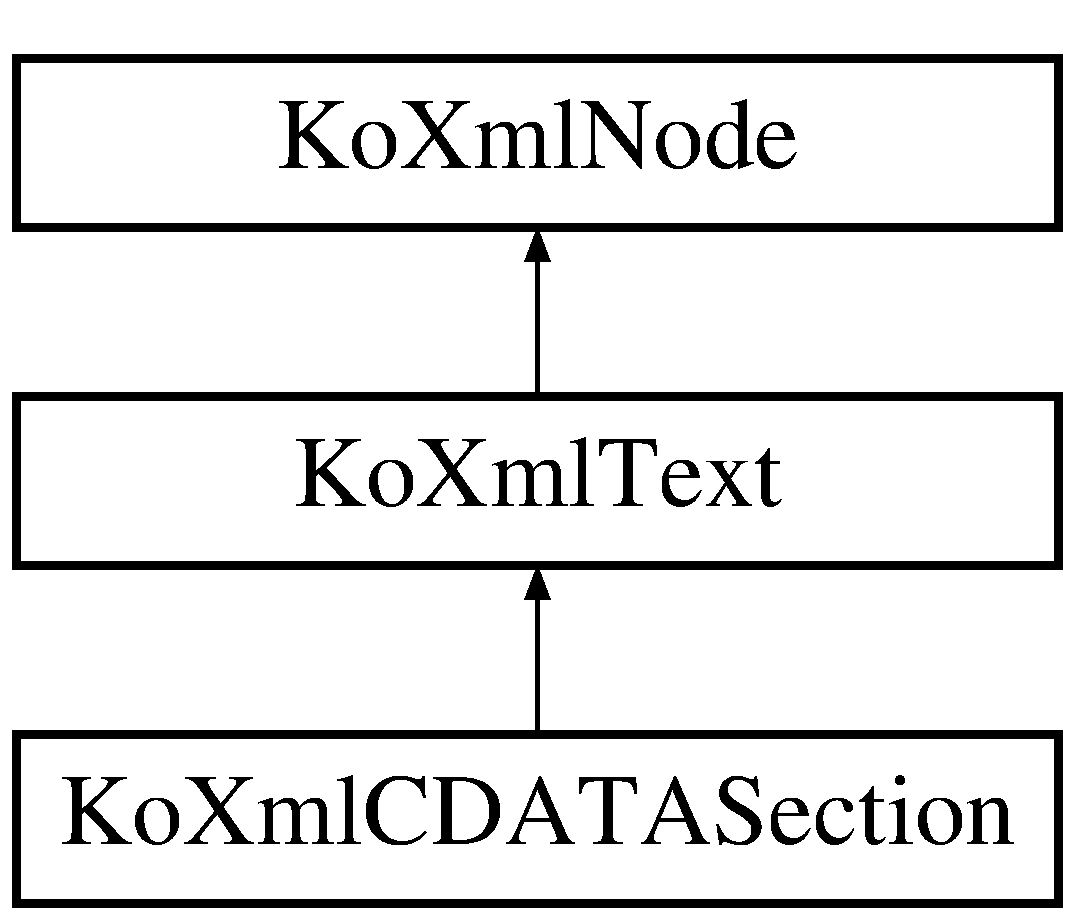
\includegraphics[height=3cm]{classKoXmlText}
\end{center}
\end{figure}
\subsection*{Public Member Functions}
\begin{DoxyCompactItemize}
\item 
\hypertarget{classKoXmlText_a527977cf8218598fc9744b55d8918dcb}{
{\bfseries KoXmlText} (const \hyperlink{classKoXmlText}{KoXmlText} \&text)}
\label{classKoXmlText_a527977cf8218598fc9744b55d8918dcb}

\item 
\hypertarget{classKoXmlText_abd7ee0d827d614bd5a387cdef944fc68}{
\hyperlink{classKoXmlText}{KoXmlText} \& {\bfseries operator=} (const \hyperlink{classKoXmlText}{KoXmlText} \&text)}
\label{classKoXmlText_abd7ee0d827d614bd5a387cdef944fc68}

\item 
\hypertarget{classKoXmlText_ab5ee4186e97c97fa2bbf54dc9ffc074f}{
QString {\bfseries data} () const }
\label{classKoXmlText_ab5ee4186e97c97fa2bbf54dc9ffc074f}

\item 
\hypertarget{classKoXmlText_a2e3b8ce0b903e43caf233d2b93ebd733}{
void {\bfseries setData} (const QString \&data)}
\label{classKoXmlText_a2e3b8ce0b903e43caf233d2b93ebd733}

\item 
\hypertarget{classKoXmlText_a910aeb556cd3a9bac84baf81899f3490}{
virtual bool {\bfseries isText} () const }
\label{classKoXmlText_a910aeb556cd3a9bac84baf81899f3490}

\end{DoxyCompactItemize}
\subsection*{Friends}
\begin{DoxyCompactItemize}
\item 
\hypertarget{classKoXmlText_a6c97883f92c7cbf2ecdf17db6cea8297}{
class \hyperlink{classKoXmlText_a6c97883f92c7cbf2ecdf17db6cea8297}{KoXmlNode}}
\label{classKoXmlText_a6c97883f92c7cbf2ecdf17db6cea8297}

\item 
\hypertarget{classKoXmlText_a50466abdb6ebb6b27c8066ac0dd926cc}{
class \hyperlink{classKoXmlText_a50466abdb6ebb6b27c8066ac0dd926cc}{KoXmlCDATASection}}
\label{classKoXmlText_a50466abdb6ebb6b27c8066ac0dd926cc}

\item 
\hypertarget{classKoXmlText_a7f0a67ef52ddc6542737225a82e4f487}{
class \hyperlink{classKoXmlText_a7f0a67ef52ddc6542737225a82e4f487}{KoXmlDocument}}
\label{classKoXmlText_a7f0a67ef52ddc6542737225a82e4f487}

\end{DoxyCompactItemize}


\subsection{Detailed Description}
\hyperlink{classKoXmlText}{KoXmlText} represents a text in a DOM tree. \begin{DoxyAuthor}{Author}
Ariya Hidayat $<$\href{mailto:ariya@kde.org}{\tt ariya@kde.org}$>$ 
\end{DoxyAuthor}


The documentation for this class was generated from the following files:\begin{DoxyCompactItemize}
\item 
src/core/KoXmlReader.h\item 
src/core/KoXmlReader.cpp\end{DoxyCompactItemize}

\hypertarget{classKoXmlWriter}{
\section{KoXmlWriter Class Reference}
\label{classKoXmlWriter}\index{KoXmlWriter@{KoXmlWriter}}
}


{\ttfamily \#include $<$KoXmlWriter.h$>$}

\subsection*{Classes}
\begin{DoxyCompactItemize}
\item 
class \hyperlink{classKoXmlWriter_1_1Private}{Private}
\item 
struct {\bfseries Tag}
\end{DoxyCompactItemize}
\subsection*{Public Member Functions}
\begin{DoxyCompactItemize}
\item 
\hyperlink{classKoXmlWriter_a533f9617e577fd34b4a4c7ad9fe23255}{KoXmlWriter} (QIODevice $\ast$dev, int indentLevel=0)
\item 
\hypertarget{classKoXmlWriter_a0af2dc9077618677116a0fe22b6f8951}{
\hyperlink{classKoXmlWriter_a0af2dc9077618677116a0fe22b6f8951}{$\sim$KoXmlWriter} ()}
\label{classKoXmlWriter_a0af2dc9077618677116a0fe22b6f8951}

\begin{DoxyCompactList}\small\item\em Destructor. \item\end{DoxyCompactList}\item 
\hypertarget{classKoXmlWriter_a43b736aa4bfa08765e0648d6fb5758ed}{
QIODevice $\ast$ {\bfseries device} () const }
\label{classKoXmlWriter_a43b736aa4bfa08765e0648d6fb5758ed}

\item 
void \hyperlink{classKoXmlWriter_a867932c8d3bbecd712572230cb0b64cd}{startDocument} (const char $\ast$rootElemName, const char $\ast$publicId=0, const char $\ast$systemId=0)
\item 
\hypertarget{classKoXmlWriter_a5ab08b557107287ecc4e1f6528a79843}{
void \hyperlink{classKoXmlWriter_a5ab08b557107287ecc4e1f6528a79843}{endDocument} ()}
\label{classKoXmlWriter_a5ab08b557107287ecc4e1f6528a79843}

\begin{DoxyCompactList}\small\item\em Call this to terminate an XML document. \item\end{DoxyCompactList}\item 
void \hyperlink{classKoXmlWriter_a38a32e955d59b3e321914320ec4f2aea}{startElement} (const char $\ast$tagName, bool indentInside=true)
\item 
void \hyperlink{classKoXmlWriter_adbe177678ee94042b4fd352245e625c6}{addAttribute} (const char $\ast$attrName, const QString \&value)
\item 
void \hyperlink{classKoXmlWriter_afa11b5f1fed349624106280436ca7fb5}{addAttribute} (const char $\ast$attrName, int value)
\item 
void \hyperlink{classKoXmlWriter_ae3103a2a23b5a037272ccae9a378d5d2}{addAttribute} (const char $\ast$attrName, uint value)
\item 
void \hyperlink{classKoXmlWriter_a70f154aa14a29bfedc6fc8a8db65274d}{addAttribute} (const char $\ast$attrName, double value)
\item 
void \hyperlink{classKoXmlWriter_af824c78438951baaad9c79cf7c1267a7}{addAttribute} (const char $\ast$attrName, float value)
\item 
void \hyperlink{classKoXmlWriter_a59281d5370c489c60515726e0b38ccd0}{addAttributePt} (const char $\ast$attrName, double value)
\item 
void \hyperlink{classKoXmlWriter_a09a850bdbc2da6652e370508d03c6395}{addAttributePt} (const char $\ast$attrName, float value)
\item 
\hypertarget{classKoXmlWriter_a146659f6c925adc68b2f2b66dccf7ac5}{
void \hyperlink{classKoXmlWriter_a146659f6c925adc68b2f2b66dccf7ac5}{addAttribute} (const char $\ast$attrName, const QByteArray \&value)}
\label{classKoXmlWriter_a146659f6c925adc68b2f2b66dccf7ac5}

\begin{DoxyCompactList}\small\item\em Overloaded version of the one taking a const char$\ast$ argument, for convenience. \item\end{DoxyCompactList}\item 
void \hyperlink{classKoXmlWriter_a920571457da436ac3c6e7f8f0521e48c}{addAttribute} (const char $\ast$attrName, const char $\ast$value)
\item 
void \hyperlink{classKoXmlWriter_ac0c62332ed7c5011e8c8edd9c26019a0}{endElement} ()
\item 
void \hyperlink{classKoXmlWriter_aabee3ed993fcc913c3466083627843fc}{addTextNode} (const QString \&str)
\item 
\hypertarget{classKoXmlWriter_a20e11dad38641d11bd1eac2f520700d3}{
void \hyperlink{classKoXmlWriter_a20e11dad38641d11bd1eac2f520700d3}{addTextNode} (const QByteArray \&cstr)}
\label{classKoXmlWriter_a20e11dad38641d11bd1eac2f520700d3}

\begin{DoxyCompactList}\small\item\em Overloaded version of the one taking a const char$\ast$ argument. \item\end{DoxyCompactList}\item 
void \hyperlink{classKoXmlWriter_a354008d8e086577751b2cbee5bf973f2}{addTextNode} (const char $\ast$cstr)
\begin{DoxyCompactList}\small\item\em Adds a text node as a child of the current element. \item\end{DoxyCompactList}\item 
void \hyperlink{classKoXmlWriter_aded4a15ee74b3dbd14cd0965d1ee471f}{addProcessingInstruction} (const char $\ast$cstr)
\begin{DoxyCompactList}\small\item\em Adds a processing instruction. \item\end{DoxyCompactList}\item 
void \hyperlink{classKoXmlWriter_acc98c1f1d995a792c7a0e4b2945954ff}{addCompleteElement} (const char $\ast$cstr)
\item 
void \hyperlink{classKoXmlWriter_a0bc25d326f56ee58c095d2e6287d6b7d}{addCompleteElement} (QIODevice $\ast$dev)
\item 
void \hyperlink{classKoXmlWriter_a168885626dde5e2432e9a2789b70715a}{addManifestEntry} (const QString \&fullPath, const QString \&mediaType)
\item 
void \hyperlink{classKoXmlWriter_aedfa20fc47c415db42871b8ff0d97e8d}{addConfigItem} (const QString \&configName, const QString \&value)
\item 
void \hyperlink{classKoXmlWriter_a2d1cc2de755ca456ca0f5bd8d81414ce}{addConfigItem} (const QString \&configName, bool value)
\item 
void \hyperlink{classKoXmlWriter_a14522a8ea1c3b25e299319653ba9af9e}{addConfigItem} (const QString \&configName, int value)
\item 
void \hyperlink{classKoXmlWriter_a3b08df454948731cdf29026298798540}{addConfigItem} (const QString \&configName, double value)
\item 
void \hyperlink{classKoXmlWriter_a3f5fa5e7f6283055cd09c94c8f67206f}{addConfigItem} (const QString \&configName, float value)
\item 
void \hyperlink{classKoXmlWriter_a96dd3ec071587e931296ce5e2b18c1e3}{addConfigItem} (const QString \&configName, long value)
\item 
void \hyperlink{classKoXmlWriter_a517c0ff99e13b5f20df48b9b49bffcca}{addConfigItem} (const QString \&configName, short value)
\item 
void \hyperlink{classKoXmlWriter_ac22324a2b86a2d5ed20026d9a47f353f}{addTextSpan} (const QString \&text)
\begin{DoxyCompactList}\small\item\em Adds a text span as nodes of the current element. \item\end{DoxyCompactList}\item 
void \hyperlink{classKoXmlWriter_a609b2173ad0698a2f6f7a9b50beb5f0d}{addTextSpan} (const QString \&text, const QMap$<$ int, int $>$ \&tabCache)
\item 
int \hyperlink{classKoXmlWriter_a71173772ef00a18d725d861cd409c0ad}{indentLevel} () const 
\item 
QList$<$ const char $\ast$ $>$ \hyperlink{classKoXmlWriter_a9b3c63f244bbf41882ea76215b1be287}{tagHierarchy} () const 
\end{DoxyCompactItemize}


\subsection{Detailed Description}
A class for writing out XML (to any QIODevice), with a special attention on performance. The XML is being written out along the way, which avoids requiring the entire document in memory (like QDom does), and avoids using QTextStream at all (which in Qt3 has major performance issues when converting to utf8). 

\subsection{Constructor \& Destructor Documentation}
\hypertarget{classKoXmlWriter_a533f9617e577fd34b4a4c7ad9fe23255}{
\index{KoXmlWriter@{KoXmlWriter}!KoXmlWriter@{KoXmlWriter}}
\index{KoXmlWriter@{KoXmlWriter}!KoXmlWriter@{KoXmlWriter}}
\subsubsection[{KoXmlWriter}]{\setlength{\rightskip}{0pt plus 5cm}KoXmlWriter::KoXmlWriter (QIODevice $\ast$ {\em dev}, \/  int {\em indentLevel} = {\ttfamily 0})\hspace{0.3cm}{\ttfamily  \mbox{[}explicit\mbox{]}}}}
\label{classKoXmlWriter_a533f9617e577fd34b4a4c7ad9fe23255}
Create a \hyperlink{classKoXmlWriter}{KoXmlWriter} instance to write out an XML document into the given QIODevice. 

\subsection{Member Function Documentation}
\hypertarget{classKoXmlWriter_a920571457da436ac3c6e7f8f0521e48c}{
\index{KoXmlWriter@{KoXmlWriter}!addAttribute@{addAttribute}}
\index{addAttribute@{addAttribute}!KoXmlWriter@{KoXmlWriter}}
\subsubsection[{addAttribute}]{\setlength{\rightskip}{0pt plus 5cm}void KoXmlWriter::addAttribute (const char $\ast$ {\em attrName}, \/  const char $\ast$ {\em value})}}
\label{classKoXmlWriter_a920571457da436ac3c6e7f8f0521e48c}
Add an attribute to the current element. \hypertarget{classKoXmlWriter_af824c78438951baaad9c79cf7c1267a7}{
\index{KoXmlWriter@{KoXmlWriter}!addAttribute@{addAttribute}}
\index{addAttribute@{addAttribute}!KoXmlWriter@{KoXmlWriter}}
\subsubsection[{addAttribute}]{\setlength{\rightskip}{0pt plus 5cm}void KoXmlWriter::addAttribute (const char $\ast$ {\em attrName}, \/  float {\em value})}}
\label{classKoXmlWriter_af824c78438951baaad9c79cf7c1267a7}
Add an attribute whose value is a floating point number The number is written out with the highest possible precision (unlike QString::number and setNum, which default to 6 digits) \hypertarget{classKoXmlWriter_a70f154aa14a29bfedc6fc8a8db65274d}{
\index{KoXmlWriter@{KoXmlWriter}!addAttribute@{addAttribute}}
\index{addAttribute@{addAttribute}!KoXmlWriter@{KoXmlWriter}}
\subsubsection[{addAttribute}]{\setlength{\rightskip}{0pt plus 5cm}void KoXmlWriter::addAttribute (const char $\ast$ {\em attrName}, \/  double {\em value})}}
\label{classKoXmlWriter_a70f154aa14a29bfedc6fc8a8db65274d}
Add an attribute whose value is a floating point number The number is written out with the highest possible precision (unlike QString::number and setNum, which default to 6 digits) \hypertarget{classKoXmlWriter_ae3103a2a23b5a037272ccae9a378d5d2}{
\index{KoXmlWriter@{KoXmlWriter}!addAttribute@{addAttribute}}
\index{addAttribute@{addAttribute}!KoXmlWriter@{KoXmlWriter}}
\subsubsection[{addAttribute}]{\setlength{\rightskip}{0pt plus 5cm}void KoXmlWriter::addAttribute (const char $\ast$ {\em attrName}, \/  uint {\em value})\hspace{0.3cm}{\ttfamily  \mbox{[}inline\mbox{]}}}}
\label{classKoXmlWriter_ae3103a2a23b5a037272ccae9a378d5d2}
Add an attribute whose value is an unsigned integer \hypertarget{classKoXmlWriter_afa11b5f1fed349624106280436ca7fb5}{
\index{KoXmlWriter@{KoXmlWriter}!addAttribute@{addAttribute}}
\index{addAttribute@{addAttribute}!KoXmlWriter@{KoXmlWriter}}
\subsubsection[{addAttribute}]{\setlength{\rightskip}{0pt plus 5cm}void KoXmlWriter::addAttribute (const char $\ast$ {\em attrName}, \/  int {\em value})\hspace{0.3cm}{\ttfamily  \mbox{[}inline\mbox{]}}}}
\label{classKoXmlWriter_afa11b5f1fed349624106280436ca7fb5}
Add an attribute whose value is an integer \hypertarget{classKoXmlWriter_adbe177678ee94042b4fd352245e625c6}{
\index{KoXmlWriter@{KoXmlWriter}!addAttribute@{addAttribute}}
\index{addAttribute@{addAttribute}!KoXmlWriter@{KoXmlWriter}}
\subsubsection[{addAttribute}]{\setlength{\rightskip}{0pt plus 5cm}void KoXmlWriter::addAttribute (const char $\ast$ {\em attrName}, \/  const QString \& {\em value})\hspace{0.3cm}{\ttfamily  \mbox{[}inline\mbox{]}}}}
\label{classKoXmlWriter_adbe177678ee94042b4fd352245e625c6}
Overloaded version of \hyperlink{classKoXmlWriter_a920571457da436ac3c6e7f8f0521e48c}{addAttribute( const char$\ast$, const char$\ast$ )}, which is a bit slower because it needs to convert {\ttfamily value} to utf8 first. \hypertarget{classKoXmlWriter_a09a850bdbc2da6652e370508d03c6395}{
\index{KoXmlWriter@{KoXmlWriter}!addAttributePt@{addAttributePt}}
\index{addAttributePt@{addAttributePt}!KoXmlWriter@{KoXmlWriter}}
\subsubsection[{addAttributePt}]{\setlength{\rightskip}{0pt plus 5cm}void KoXmlWriter::addAttributePt (const char $\ast$ {\em attrName}, \/  float {\em value})}}
\label{classKoXmlWriter_a09a850bdbc2da6652e370508d03c6395}
Add an attribute which represents a distance, measured in pt The number is written out with the highest possible precision (unlike QString::number and setNum, which default to 6 digits), and the unit name (\char`\"{}pt\char`\"{}) is appended to it. \hypertarget{classKoXmlWriter_a59281d5370c489c60515726e0b38ccd0}{
\index{KoXmlWriter@{KoXmlWriter}!addAttributePt@{addAttributePt}}
\index{addAttributePt@{addAttributePt}!KoXmlWriter@{KoXmlWriter}}
\subsubsection[{addAttributePt}]{\setlength{\rightskip}{0pt plus 5cm}void KoXmlWriter::addAttributePt (const char $\ast$ {\em attrName}, \/  double {\em value})}}
\label{classKoXmlWriter_a59281d5370c489c60515726e0b38ccd0}
Add an attribute which represents a distance, measured in pt The number is written out with the highest possible precision (unlike QString::number and setNum, which default to 6 digits), and the unit name (\char`\"{}pt\char`\"{}) is appended to it. \hypertarget{classKoXmlWriter_a0bc25d326f56ee58c095d2e6287d6b7d}{
\index{KoXmlWriter@{KoXmlWriter}!addCompleteElement@{addCompleteElement}}
\index{addCompleteElement@{addCompleteElement}!KoXmlWriter@{KoXmlWriter}}
\subsubsection[{addCompleteElement}]{\setlength{\rightskip}{0pt plus 5cm}void KoXmlWriter::addCompleteElement (QIODevice $\ast$ {\em dev})}}
\label{classKoXmlWriter_a0bc25d326f56ee58c095d2e6287d6b7d}
This is quite a special-\/purpose method, not for everyday use. It adds a complete element (with its attributes and child elements) as a child of the current element. The iodevice is supposed to be escaped for XML already, so it will usually come from another \hyperlink{classKoXmlWriter}{KoXmlWriter}. This is usually used with KTempFile. \hypertarget{classKoXmlWriter_acc98c1f1d995a792c7a0e4b2945954ff}{
\index{KoXmlWriter@{KoXmlWriter}!addCompleteElement@{addCompleteElement}}
\index{addCompleteElement@{addCompleteElement}!KoXmlWriter@{KoXmlWriter}}
\subsubsection[{addCompleteElement}]{\setlength{\rightskip}{0pt plus 5cm}void KoXmlWriter::addCompleteElement (const char $\ast$ {\em cstr})}}
\label{classKoXmlWriter_acc98c1f1d995a792c7a0e4b2945954ff}
This is quite a special-\/purpose method, not for everyday use. It adds a complete element (with its attributes and child elements) as a child of the current element. The string is supposed to be escaped for XML already, so it will usually come from another \hyperlink{classKoXmlWriter}{KoXmlWriter}. \hypertarget{classKoXmlWriter_a517c0ff99e13b5f20df48b9b49bffcca}{
\index{KoXmlWriter@{KoXmlWriter}!addConfigItem@{addConfigItem}}
\index{addConfigItem@{addConfigItem}!KoXmlWriter@{KoXmlWriter}}
\subsubsection[{addConfigItem}]{\setlength{\rightskip}{0pt plus 5cm}void KoXmlWriter::addConfigItem (const QString \& {\em configName}, \/  short {\em value})}}
\label{classKoXmlWriter_a517c0ff99e13b5f20df48b9b49bffcca}
\begin{DoxyNote}{Note}
OASIS-\/specific 
\end{DoxyNote}
\hypertarget{classKoXmlWriter_a96dd3ec071587e931296ce5e2b18c1e3}{
\index{KoXmlWriter@{KoXmlWriter}!addConfigItem@{addConfigItem}}
\index{addConfigItem@{addConfigItem}!KoXmlWriter@{KoXmlWriter}}
\subsubsection[{addConfigItem}]{\setlength{\rightskip}{0pt plus 5cm}void KoXmlWriter::addConfigItem (const QString \& {\em configName}, \/  long {\em value})}}
\label{classKoXmlWriter_a96dd3ec071587e931296ce5e2b18c1e3}
\begin{DoxyNote}{Note}
OASIS-\/specific 
\end{DoxyNote}
\hypertarget{classKoXmlWriter_a3f5fa5e7f6283055cd09c94c8f67206f}{
\index{KoXmlWriter@{KoXmlWriter}!addConfigItem@{addConfigItem}}
\index{addConfigItem@{addConfigItem}!KoXmlWriter@{KoXmlWriter}}
\subsubsection[{addConfigItem}]{\setlength{\rightskip}{0pt plus 5cm}void KoXmlWriter::addConfigItem (const QString \& {\em configName}, \/  float {\em value})}}
\label{classKoXmlWriter_a3f5fa5e7f6283055cd09c94c8f67206f}
\begin{DoxyNote}{Note}
OASIS-\/specific 
\end{DoxyNote}
\hypertarget{classKoXmlWriter_a3b08df454948731cdf29026298798540}{
\index{KoXmlWriter@{KoXmlWriter}!addConfigItem@{addConfigItem}}
\index{addConfigItem@{addConfigItem}!KoXmlWriter@{KoXmlWriter}}
\subsubsection[{addConfigItem}]{\setlength{\rightskip}{0pt plus 5cm}void KoXmlWriter::addConfigItem (const QString \& {\em configName}, \/  double {\em value})}}
\label{classKoXmlWriter_a3b08df454948731cdf29026298798540}
\begin{DoxyNote}{Note}
OASIS-\/specific 
\end{DoxyNote}
\hypertarget{classKoXmlWriter_a14522a8ea1c3b25e299319653ba9af9e}{
\index{KoXmlWriter@{KoXmlWriter}!addConfigItem@{addConfigItem}}
\index{addConfigItem@{addConfigItem}!KoXmlWriter@{KoXmlWriter}}
\subsubsection[{addConfigItem}]{\setlength{\rightskip}{0pt plus 5cm}void KoXmlWriter::addConfigItem (const QString \& {\em configName}, \/  int {\em value})}}
\label{classKoXmlWriter_a14522a8ea1c3b25e299319653ba9af9e}
\begin{DoxyNote}{Note}
OASIS-\/specific 
\end{DoxyNote}
\hypertarget{classKoXmlWriter_a2d1cc2de755ca456ca0f5bd8d81414ce}{
\index{KoXmlWriter@{KoXmlWriter}!addConfigItem@{addConfigItem}}
\index{addConfigItem@{addConfigItem}!KoXmlWriter@{KoXmlWriter}}
\subsubsection[{addConfigItem}]{\setlength{\rightskip}{0pt plus 5cm}void KoXmlWriter::addConfigItem (const QString \& {\em configName}, \/  bool {\em value})}}
\label{classKoXmlWriter_a2d1cc2de755ca456ca0f5bd8d81414ce}
\begin{DoxyNote}{Note}
OASIS-\/specific 
\end{DoxyNote}
\hypertarget{classKoXmlWriter_aedfa20fc47c415db42871b8ff0d97e8d}{
\index{KoXmlWriter@{KoXmlWriter}!addConfigItem@{addConfigItem}}
\index{addConfigItem@{addConfigItem}!KoXmlWriter@{KoXmlWriter}}
\subsubsection[{addConfigItem}]{\setlength{\rightskip}{0pt plus 5cm}void KoXmlWriter::addConfigItem (const QString \& {\em configName}, \/  const QString \& {\em value})}}
\label{classKoXmlWriter_aedfa20fc47c415db42871b8ff0d97e8d}
Special helper for writing config item into settings.xml \begin{DoxyNote}{Note}
OASIS-\/specific 
\end{DoxyNote}
\hypertarget{classKoXmlWriter_a168885626dde5e2432e9a2789b70715a}{
\index{KoXmlWriter@{KoXmlWriter}!addManifestEntry@{addManifestEntry}}
\index{addManifestEntry@{addManifestEntry}!KoXmlWriter@{KoXmlWriter}}
\subsubsection[{addManifestEntry}]{\setlength{\rightskip}{0pt plus 5cm}void KoXmlWriter::addManifestEntry (const QString \& {\em fullPath}, \/  const QString \& {\em mediaType})}}
\label{classKoXmlWriter_a168885626dde5e2432e9a2789b70715a}
Special helper for writing \char`\"{}manifest\char`\"{} files This is equivalent to startElement/2$\ast$addAttribute/endElement This API will probably have to change (or not be used anymore) when we add support for encrypting/signing. \begin{DoxyNote}{Note}
OASIS-\/specific 
\end{DoxyNote}
\hypertarget{classKoXmlWriter_aded4a15ee74b3dbd14cd0965d1ee471f}{
\index{KoXmlWriter@{KoXmlWriter}!addProcessingInstruction@{addProcessingInstruction}}
\index{addProcessingInstruction@{addProcessingInstruction}!KoXmlWriter@{KoXmlWriter}}
\subsubsection[{addProcessingInstruction}]{\setlength{\rightskip}{0pt plus 5cm}void KoXmlWriter::addProcessingInstruction (const char $\ast$ {\em cstr})}}
\label{classKoXmlWriter_aded4a15ee74b3dbd14cd0965d1ee471f}


Adds a processing instruction. 

This writes a processing instruction, like $<$?foo bar blah?$>$, where foo is the target, and the rest is the data.

Processing instructions are used in XML to keep processor-\/specific information in the text of the document. \hypertarget{classKoXmlWriter_a354008d8e086577751b2cbee5bf973f2}{
\index{KoXmlWriter@{KoXmlWriter}!addTextNode@{addTextNode}}
\index{addTextNode@{addTextNode}!KoXmlWriter@{KoXmlWriter}}
\subsubsection[{addTextNode}]{\setlength{\rightskip}{0pt plus 5cm}void KoXmlWriter::addTextNode (const char $\ast$ {\em cstr})}}
\label{classKoXmlWriter_a354008d8e086577751b2cbee5bf973f2}


Adds a text node as a child of the current element. 

This is appends the literal content of {\ttfamily str} to the contents of the element. E.g. addTextNode( \char`\"{}foo\char`\"{} ) inside a $<$p$>$ element gives $<$p$>$foo$<$/p$>$, and startElement( \char`\"{}b\char`\"{} ); endElement( \char`\"{}b\char`\"{} ); addTextNode( \char`\"{}foo\char`\"{} ) gives $<$p$>$$<$b/$>$foo$<$/p$>$ \hypertarget{classKoXmlWriter_aabee3ed993fcc913c3466083627843fc}{
\index{KoXmlWriter@{KoXmlWriter}!addTextNode@{addTextNode}}
\index{addTextNode@{addTextNode}!KoXmlWriter@{KoXmlWriter}}
\subsubsection[{addTextNode}]{\setlength{\rightskip}{0pt plus 5cm}void KoXmlWriter::addTextNode (const QString \& {\em str})\hspace{0.3cm}{\ttfamily  \mbox{[}inline\mbox{]}}}}
\label{classKoXmlWriter_aabee3ed993fcc913c3466083627843fc}
Overloaded version of \hyperlink{classKoXmlWriter_a354008d8e086577751b2cbee5bf973f2}{addTextNode( const char$\ast$ )}, which is a bit slower because it needs to convert {\ttfamily str} to utf8 first. \hypertarget{classKoXmlWriter_a609b2173ad0698a2f6f7a9b50beb5f0d}{
\index{KoXmlWriter@{KoXmlWriter}!addTextSpan@{addTextSpan}}
\index{addTextSpan@{addTextSpan}!KoXmlWriter@{KoXmlWriter}}
\subsubsection[{addTextSpan}]{\setlength{\rightskip}{0pt plus 5cm}void KoXmlWriter::addTextSpan (const QString \& {\em text}, \/  const QMap$<$ int, int $>$ \& {\em tabCache})}}
\label{classKoXmlWriter_a609b2173ad0698a2f6f7a9b50beb5f0d}
Overloaded version of addTextSpan which takes an additional tabCache map. 
\begin{DoxyParams}{Parameters}
\item[{\em text}]the text to write \item[{\em tabCache}]optional map allowing to find a tab for a given character index \end{DoxyParams}
\begin{DoxyNote}{Note}
OASIS-\/specific 
\end{DoxyNote}
\hypertarget{classKoXmlWriter_ac22324a2b86a2d5ed20026d9a47f353f}{
\index{KoXmlWriter@{KoXmlWriter}!addTextSpan@{addTextSpan}}
\index{addTextSpan@{addTextSpan}!KoXmlWriter@{KoXmlWriter}}
\subsubsection[{addTextSpan}]{\setlength{\rightskip}{0pt plus 5cm}void KoXmlWriter::addTextSpan (const QString \& {\em text})}}
\label{classKoXmlWriter_ac22324a2b86a2d5ed20026d9a47f353f}


Adds a text span as nodes of the current element. 

Unlike \hyperlink{classKoXmlWriter_aabee3ed993fcc913c3466083627843fc}{KoXmlWriter::addTextNode} it handles tabulations, linebreaks, and multiple spaces by using the appropriate OASIS tags.


\begin{DoxyParams}{Parameters}
\item[{\em text}]the text to write\end{DoxyParams}
\begin{DoxyNote}{Note}
OASIS-\/specific 
\end{DoxyNote}
\hypertarget{classKoXmlWriter_ac0c62332ed7c5011e8c8edd9c26019a0}{
\index{KoXmlWriter@{KoXmlWriter}!endElement@{endElement}}
\index{endElement@{endElement}!KoXmlWriter@{KoXmlWriter}}
\subsubsection[{endElement}]{\setlength{\rightskip}{0pt plus 5cm}void KoXmlWriter::endElement ()}}
\label{classKoXmlWriter_ac0c62332ed7c5011e8c8edd9c26019a0}
Terminate the current element. After this you should start a new one (sibling), add a sibling text node, or close another one (end of siblings). \hypertarget{classKoXmlWriter_a71173772ef00a18d725d861cd409c0ad}{
\index{KoXmlWriter@{KoXmlWriter}!indentLevel@{indentLevel}}
\index{indentLevel@{indentLevel}!KoXmlWriter@{KoXmlWriter}}
\subsubsection[{indentLevel}]{\setlength{\rightskip}{0pt plus 5cm}int KoXmlWriter::indentLevel () const}}
\label{classKoXmlWriter_a71173772ef00a18d725d861cd409c0ad}
\begin{DoxyReturn}{Returns}
the current indentation level. Useful when creating a sub-\/KoXmlWriter (see addCompleteElement) 
\end{DoxyReturn}
\hypertarget{classKoXmlWriter_a867932c8d3bbecd712572230cb0b64cd}{
\index{KoXmlWriter@{KoXmlWriter}!startDocument@{startDocument}}
\index{startDocument@{startDocument}!KoXmlWriter@{KoXmlWriter}}
\subsubsection[{startDocument}]{\setlength{\rightskip}{0pt plus 5cm}void KoXmlWriter::startDocument (const char $\ast$ {\em rootElemName}, \/  const char $\ast$ {\em publicId} = {\ttfamily 0}, \/  const char $\ast$ {\em systemId} = {\ttfamily 0})}}
\label{classKoXmlWriter_a867932c8d3bbecd712572230cb0b64cd}
Start the XML document. This writes out the $<$?xml?$>$ tag with utf8 encoding, and the DOCTYPE. 
\begin{DoxyParams}{Parameters}
\item[{\em rootElemName}]the name of the root element, used in the DOCTYPE tag. \item[{\em publicId}]the public identifier, e.g. \char`\"{}-\///OpenOffice.org//DTD OfficeDocument 1.0//EN\char`\"{} \item[{\em systemId}]the system identifier, e.g. \char`\"{}office.dtd\char`\"{} or a full URL to it. \end{DoxyParams}
\hypertarget{classKoXmlWriter_a38a32e955d59b3e321914320ec4f2aea}{
\index{KoXmlWriter@{KoXmlWriter}!startElement@{startElement}}
\index{startElement@{startElement}!KoXmlWriter@{KoXmlWriter}}
\subsubsection[{startElement}]{\setlength{\rightskip}{0pt plus 5cm}void KoXmlWriter::startElement (const char $\ast$ {\em tagName}, \/  bool {\em indentInside} = {\ttfamily true})}}
\label{classKoXmlWriter_a38a32e955d59b3e321914320ec4f2aea}
Start a new element, as a child of the current element. 
\begin{DoxyParams}{Parameters}
\item[{\em tagName}]the name of the tag. Warning: this string must remain alive until endElement, no copy is internally made. Usually tagName is a string constant so this is no problem anyway. \item[{\em indentInside}]if set to false, there will be no indentation inside this tag. This is useful for elements where whitespace matters. \end{DoxyParams}
\hypertarget{classKoXmlWriter_a9b3c63f244bbf41882ea76215b1be287}{
\index{KoXmlWriter@{KoXmlWriter}!tagHierarchy@{tagHierarchy}}
\index{tagHierarchy@{tagHierarchy}!KoXmlWriter@{KoXmlWriter}}
\subsubsection[{tagHierarchy}]{\setlength{\rightskip}{0pt plus 5cm}QList$<$ const char $\ast$ $>$ KoXmlWriter::tagHierarchy () const}}
\label{classKoXmlWriter_a9b3c63f244bbf41882ea76215b1be287}
Return all the open tags at this time, root element first. 

The documentation for this class was generated from the following files:\begin{DoxyCompactItemize}
\item 
src/core/KoXmlWriter.h\item 
src/core/KoXmlWriter.cpp\end{DoxyCompactItemize}

\hypertarget{classMainWindow}{
\section{MainWindow Class Reference}
\label{classMainWindow}\index{MainWindow@{MainWindow}}
}
\subsection*{Public Slots}
\begin{DoxyCompactItemize}
\item 
\hypertarget{classMainWindow_ac4d16cb0945152f7be27dcac8f85703d}{
void {\bfseries showSettingsDialog\_\-Module} ()}
\label{classMainWindow_ac4d16cb0945152f7be27dcac8f85703d}

\item 
\hypertarget{classMainWindow_a1c14a341d9d6b8c3b76d7c4a838463d8}{
void {\bfseries showSettingsDialog\_\-General} ()}
\label{classMainWindow_a1c14a341d9d6b8c3b76d7c4a838463d8}

\item 
\hypertarget{classMainWindow_adcb5fb16f13d14efcf2d8c37cb44d732}{
void {\bfseries saveSettings} (\hyperlink{classSettings}{Settings} set)}
\label{classMainWindow_adcb5fb16f13d14efcf2d8c37cb44d732}

\end{DoxyCompactItemize}
\subsection*{Signals}
\begin{DoxyCompactItemize}
\item 
\hypertarget{classMainWindow_aa5579ecfd0f160021551ba302e122149}{
void {\bfseries settingsChanged} (\hyperlink{classSettings}{Settings} settings)}
\label{classMainWindow_aa5579ecfd0f160021551ba302e122149}

\item 
\hypertarget{classMainWindow_ac03d41a0c3906055917074addf64403b}{
void {\bfseries closing} ()}
\label{classMainWindow_ac03d41a0c3906055917074addf64403b}

\end{DoxyCompactItemize}
\subsection*{Public Member Functions}
\begin{DoxyCompactItemize}
\item 
\hypertarget{classMainWindow_a8b244be8b7b7db1b08de2a2acb9409db}{
{\bfseries MainWindow} (QWidget $\ast$parent=0)}
\label{classMainWindow_a8b244be8b7b7db1b08de2a2acb9409db}

\item 
\hypertarget{classMainWindow_a1f508b9d9a5a263923fb3cc8fc9972b7}{
void {\bfseries init} (const QString \&homeDataPath)}
\label{classMainWindow_a1f508b9d9a5a263923fb3cc8fc9972b7}

\item 
\hypertarget{classMainWindow_abd169790e33b6568ba2229df1d4b4e51}{
void {\bfseries loadSimpleInterface} ()}
\label{classMainWindow_abd169790e33b6568ba2229df1d4b4e51}

\item 
\hypertarget{classMainWindow_a497461898e28b50f19b7c5c635fb0a40}{
void {\bfseries loadAdvancedInterface} ()}
\label{classMainWindow_a497461898e28b50f19b7c5c635fb0a40}

\item 
\hypertarget{classMainWindow_adfdcb49e4eabc699c5893a4612d2c627}{
void {\bfseries loadStudyInterface} ()}
\label{classMainWindow_adfdcb49e4eabc699c5893a4612d2c627}

\item 
\hypertarget{classMainWindow_a9b9a4d029dead797c739cb67dffc1b54}{
void {\bfseries loadDefaultSettings} ()}
\label{classMainWindow_a9b9a4d029dead797c739cb67dffc1b54}

\item 
\hypertarget{classMainWindow_a9bb1f3b7f6b5360abfd2dc01fc1c8930}{
void {\bfseries loadSettings} ()}
\label{classMainWindow_a9bb1f3b7f6b5360abfd2dc01fc1c8930}

\item 
\hypertarget{classMainWindow_a10f2072278f64aa75a70cc4aa5cd2db7}{
void {\bfseries restoreSession} ()}
\label{classMainWindow_a10f2072278f64aa75a70cc4aa5cd2db7}

\item 
\hypertarget{classMainWindow_a2daa5870beeb252bbab6ce99c072e339}{
void {\bfseries setSettings} (\hyperlink{classSettings}{Settings} $\ast$setttings)}
\label{classMainWindow_a2daa5870beeb252bbab6ce99c072e339}

\item 
\hypertarget{classMainWindow_af03afe1c5ec6d2af47478b31f241a598}{
void {\bfseries setSettings} (\hyperlink{classSettings}{Settings} settings)}
\label{classMainWindow_af03afe1c5ec6d2af47478b31f241a598}

\item 
\hypertarget{classMainWindow_a49be45fc9b993fdc3afe55d4b6fa0650}{
void {\bfseries writeSettings} ()}
\label{classMainWindow_a49be45fc9b993fdc3afe55d4b6fa0650}

\item 
\hypertarget{classMainWindow_a7059d33161e3004eeb67831af59764d3}{
void {\bfseries showSettingsDialog} (int tabID)}
\label{classMainWindow_a7059d33161e3004eeb67831af59764d3}

\item 
\hypertarget{classMainWindow_a7e23764f34b4f77bff2e668d3af32585}{
void {\bfseries loadLanguage} (QString language)}
\label{classMainWindow_a7e23764f34b4f77bff2e668d3af32585}

\item 
\hypertarget{classMainWindow_a36c558b2a34c0bb56ae8a60c5bcfdff0}{
void {\bfseries setTranslator} (QTranslator $\ast$my, QTranslator $\ast$qt)}
\label{classMainWindow_a36c558b2a34c0bb56ae8a60c5bcfdff0}

\end{DoxyCompactItemize}
\subsection*{Public Attributes}
\begin{DoxyCompactItemize}
\item 
\hypertarget{classMainWindow_ad0cd93fa38bb5ec71d8973ac66af2615}{
\hyperlink{classModuleManager}{ModuleManager} $\ast$ {\bfseries m\_\-moduleManager}}
\label{classMainWindow_ad0cd93fa38bb5ec71d8973ac66af2615}

\item 
\hypertarget{classMainWindow_a192b3d658f9ef44b532a66ac4b375176}{
\hyperlink{classBibleDisplay}{BibleDisplay} $\ast$ {\bfseries m\_\-bibleDisplay}}
\label{classMainWindow_a192b3d658f9ef44b532a66ac4b375176}

\item 
\hypertarget{classMainWindow_ae5f31d6baa938f1fdf33694bb36501bc}{
\hyperlink{classSettings}{Settings} $\ast$ {\bfseries m\_\-settings}}
\label{classMainWindow_ae5f31d6baa938f1fdf33694bb36501bc}

\item 
\hypertarget{classMainWindow_a0a0315b93be2c938662a02e1d813cf49}{
\hyperlink{classNotes}{Notes} $\ast$ {\bfseries m\_\-notes}}
\label{classMainWindow_a0a0315b93be2c938662a02e1d813cf49}

\item 
\hypertarget{classMainWindow_aca0fe0d96000882083d46631d79e950d}{
\hyperlink{classSession}{Session} $\ast$ {\bfseries m\_\-session}}
\label{classMainWindow_aca0fe0d96000882083d46631d79e950d}

\item 
\hypertarget{classMainWindow_a77fe7254ab86dd608773a14e47c46107}{
QSettings $\ast$ {\bfseries m\_\-settingsFile}}
\label{classMainWindow_a77fe7254ab86dd608773a14e47c46107}

\item 
\hypertarget{classMainWindow_a3a92e4812a8695f1eb366a4fcad5015a}{
QString {\bfseries VERSION}}
\label{classMainWindow_a3a92e4812a8695f1eb366a4fcad5015a}

\item 
\hypertarget{classMainWindow_a52a9752c79e2f4e23aaf8e83fdcc73f9}{
QString {\bfseries BUILD}}
\label{classMainWindow_a52a9752c79e2f4e23aaf8e83fdcc73f9}

\item 
\hypertarget{classMainWindow_abb8d42b6e667d979f29b5198fe7a1d9f}{
QString {\bfseries m\_\-homeDataPath}}
\label{classMainWindow_abb8d42b6e667d979f29b5198fe7a1d9f}

\item 
\hypertarget{classMainWindow_a9715e4f3c6516a29086cbeab4d24e4b9}{
QTranslator $\ast$ {\bfseries myappTranslator}}
\label{classMainWindow_a9715e4f3c6516a29086cbeab4d24e4b9}

\item 
\hypertarget{classMainWindow_a24d77db9a9c7cd5239866e356ccfe280}{
QTranslator $\ast$ {\bfseries qtTranslator}}
\label{classMainWindow_a24d77db9a9c7cd5239866e356ccfe280}

\end{DoxyCompactItemize}
\subsection*{Protected Member Functions}
\begin{DoxyCompactItemize}
\item 
\hypertarget{classMainWindow_af4ca5d0d3d18ddcb7d54b6596bbf4797}{
void {\bfseries changeEvent} (QEvent $\ast$e)}
\label{classMainWindow_af4ca5d0d3d18ddcb7d54b6596bbf4797}

\item 
\hypertarget{classMainWindow_a4e20a4a065fbb0e4d3532a45a0a91425}{
void {\bfseries closeEvent} (QCloseEvent $\ast$event)}
\label{classMainWindow_a4e20a4a065fbb0e4d3532a45a0a91425}

\end{DoxyCompactItemize}


The documentation for this class was generated from the following files:\begin{DoxyCompactItemize}
\item 
src/ui/mainwindow.h\item 
src/ui/mainwindow.cpp\end{DoxyCompactItemize}

\hypertarget{classModuleConfigDialog}{
\section{ModuleConfigDialog Class Reference}
\label{classModuleConfigDialog}\index{ModuleConfigDialog@{ModuleConfigDialog}}
}


{\ttfamily \#include $<$moduleconfigdialog.h$>$}

\subsection*{Signals}
\begin{DoxyCompactItemize}
\item 
\hypertarget{classModuleConfigDialog_a84f3addff3fdb1f9ceac5efad6a21c37}{
void {\bfseries save} (\hyperlink{classModuleSettings}{ModuleSettings} config)}
\label{classModuleConfigDialog_a84f3addff3fdb1f9ceac5efad6a21c37}

\end{DoxyCompactItemize}
\subsection*{Public Member Functions}
\begin{DoxyCompactItemize}
\item 
\hypertarget{classModuleConfigDialog_aeb291f87e7e3749701299118e521ddc0}{
{\bfseries ModuleConfigDialog} (QWidget $\ast$parent=0)}
\label{classModuleConfigDialog_aeb291f87e7e3749701299118e521ddc0}

\item 
\hypertarget{classModuleConfigDialog_aa66110dc25bdd33d6b5960b87e15beb1}{
void {\bfseries setModule} (\hyperlink{classModuleSettings}{ModuleSettings} config)}
\label{classModuleConfigDialog_aa66110dc25bdd33d6b5960b87e15beb1}

\end{DoxyCompactItemize}
\subsection*{Protected Member Functions}
\begin{DoxyCompactItemize}
\item 
\hypertarget{classModuleConfigDialog_a0eeda84ed46ffc60b77183542eb4f583}{
virtual void {\bfseries changeEvent} (QEvent $\ast$e)}
\label{classModuleConfigDialog_a0eeda84ed46ffc60b77183542eb4f583}

\end{DoxyCompactItemize}


\subsection{Detailed Description}
\hyperlink{classModuleConfigDialog}{ModuleConfigDialog} represents a dialog to change module settings 

The documentation for this class was generated from the following files:\begin{DoxyCompactItemize}
\item 
src/ui/dialog/moduleconfigdialog.h\item 
src/ui/dialog/moduleconfigdialog.cpp\end{DoxyCompactItemize}

\hypertarget{classModuleDownloadDialog}{
\section{ModuleDownloadDialog Class Reference}
\label{classModuleDownloadDialog}\index{ModuleDownloadDialog@{ModuleDownloadDialog}}
}


{\ttfamily \#include $<$moduledownloaddialog.h$>$}

\subsection*{Signals}
\begin{DoxyCompactItemize}
\item 
\hypertarget{classModuleDownloadDialog_a285d9619e209258c79f40dc34b8682d4}{
void {\bfseries downloaded} (QStringList downloadedFiles, QStringList names)}
\label{classModuleDownloadDialog_a285d9619e209258c79f40dc34b8682d4}

\end{DoxyCompactItemize}
\subsection*{Public Member Functions}
\begin{DoxyCompactItemize}
\item 
\hypertarget{classModuleDownloadDialog_a893c5c6dfa7680361af886502a0f80e3}{
{\bfseries ModuleDownloadDialog} (QWidget $\ast$parent=0)}
\label{classModuleDownloadDialog_a893c5c6dfa7680361af886502a0f80e3}

\item 
\hypertarget{classModuleDownloadDialog_a471587fb7073ab5113bfed9f46aca5f7}{
void {\bfseries setSettings} (\hyperlink{classSettings}{Settings} settings)}
\label{classModuleDownloadDialog_a471587fb7073ab5113bfed9f46aca5f7}

\item 
\hypertarget{classModuleDownloadDialog_af63cad20b2af821018617fb49f2c3e77}{
void {\bfseries readModules} ()}
\label{classModuleDownloadDialog_af63cad20b2af821018617fb49f2c3e77}

\end{DoxyCompactItemize}
\subsection*{Protected Member Functions}
\begin{DoxyCompactItemize}
\item 
\hypertarget{classModuleDownloadDialog_a6b1d8ab0687323e33b28ed53a9f1f341}{
void {\bfseries changeEvent} (QEvent $\ast$e)}
\label{classModuleDownloadDialog_a6b1d8ab0687323e33b28ed53a9f1f341}

\end{DoxyCompactItemize}


\subsection{Detailed Description}
\hyperlink{classModuleDownloadDialog}{ModuleDownloadDialog} represents a dialog to download new modules 

The documentation for this class was generated from the following files:\begin{DoxyCompactItemize}
\item 
src/ui/dialog/moduledownloaddialog.h\item 
src/ui/dialog/moduledownloaddialog.cpp\end{DoxyCompactItemize}

\hypertarget{classModuleSettings}{
\section{ModuleSettings Class Reference}
\label{classModuleSettings}\index{ModuleSettings@{ModuleSettings}}
}


{\ttfamily \#include $<$modulesettings.h$>$}

\subsection*{Public Attributes}
\begin{DoxyCompactItemize}
\item 
\hypertarget{classModuleSettings_aa408aa93b659f03f91d66e742c56c39c}{
QString {\bfseries modulePath}}
\label{classModuleSettings_aa408aa93b659f03f91d66e742c56c39c}

\item 
\hypertarget{classModuleSettings_acf1a856fdf42a2ceee420d478a272256}{
QString {\bfseries moduleName}}
\label{classModuleSettings_acf1a856fdf42a2ceee420d478a272256}

\item 
\hypertarget{classModuleSettings_aa5aa01e89cd61f4b19134b0d5d372034}{
QString {\bfseries moduleType}}
\label{classModuleSettings_aa5aa01e89cd61f4b19134b0d5d372034}

\item 
\hypertarget{classModuleSettings_a0c0bb115443c382e54e406aa1a0ecce2}{
QString {\bfseries encoding}}
\label{classModuleSettings_a0c0bb115443c382e54e406aa1a0ecce2}

\item 
\hypertarget{classModuleSettings_a8609fa8d6e05485f136ede4b7497d393}{
bool {\bfseries isDir}}
\label{classModuleSettings_a8609fa8d6e05485f136ede4b7497d393}

\item 
\hypertarget{classModuleSettings_ae48c0b3d62cf6e20b6ecf6d2c9df46bb}{
int {\bfseries zefbible\_\-textFormatting}}
\label{classModuleSettings_ae48c0b3d62cf6e20b6ecf6d2c9df46bb}

\item 
\hypertarget{classModuleSettings_a3a2e80afc1f966db21ef5fb326dbdf7f}{
bool {\bfseries zefbible\_\-hardCache}}
\label{classModuleSettings_a3a2e80afc1f966db21ef5fb326dbdf7f}

\item 
\hypertarget{classModuleSettings_a457dcb021bbe45a905fd66e0e92c9435}{
bool {\bfseries zefbible\_\-softCache}}
\label{classModuleSettings_a457dcb021bbe45a905fd66e0e92c9435}

\item 
\hypertarget{classModuleSettings_a511bd56eead503c3be216489066f100f}{
bool {\bfseries zefbible\_\-showStrong}}
\label{classModuleSettings_a511bd56eead503c3be216489066f100f}

\item 
\hypertarget{classModuleSettings_a855e48f769627a54b2643a872e5838ac}{
bool {\bfseries zefbible\_\-showStudyNote}}
\label{classModuleSettings_a855e48f769627a54b2643a872e5838ac}

\item 
\hypertarget{classModuleSettings_a8fd9c1bd55ee42af5ee9b24e4fe6ee92}{
bool {\bfseries biblequote\_\-removeHtml}}
\label{classModuleSettings_a8fd9c1bd55ee42af5ee9b24e4fe6ee92}

\item 
\hypertarget{classModuleSettings_ae1c590d226d0b7c994f1b2cc85de342e}{
int {\bfseries uModuleCount}}
\label{classModuleSettings_ae1c590d226d0b7c994f1b2cc85de342e}

\item 
\hypertarget{classModuleSettings_a4b1acf7fab7f33a9daa83a6043216d75}{
QMap$<$ QString, QVariant $>$ {\bfseries bookCount}}
\label{classModuleSettings_a4b1acf7fab7f33a9daa83a6043216d75}

\item 
\hypertarget{classModuleSettings_a8e111bc80c36144142f2249d58d8be0f}{
QMap$<$ QString, QVariant $>$ {\bfseries bookNames}}
\label{classModuleSettings_a8e111bc80c36144142f2249d58d8be0f}

\item 
\hypertarget{classModuleSettings_a40622a8984b16c59c645a304f6c7b3d6}{
QMap$<$ QString, QVariant $>$ {\bfseries biblePath}}
\label{classModuleSettings_a40622a8984b16c59c645a304f6c7b3d6}

\item 
\hypertarget{classModuleSettings_aa5a936a337616dc4edcc2b2b4dbeaae8}{
QMap$<$ QString, QVariant $>$ {\bfseries bibleName}}
\label{classModuleSettings_aa5a936a337616dc4edcc2b2b4dbeaae8}

\end{DoxyCompactItemize}


\subsection{Detailed Description}
\hyperlink{classModuleSettings}{ModuleSettings} represents a settings class for modules

\begin{DoxyAuthor}{Author}
Paul Walger $<$\href{mailto:metaxy@walger.name}{\tt metaxy@walger.name}$>$ 
\end{DoxyAuthor}


The documentation for this class was generated from the following files:\begin{DoxyCompactItemize}
\item 
src/core/modulesettings.h\item 
src/core/modulesettings.cpp\end{DoxyCompactItemize}

\hypertarget{classNotes}{
\section{Notes Class Reference}
\label{classNotes}\index{Notes@{Notes}}
}


{\ttfamily \#include $<$notes.h$>$}\subsection*{Public Member Functions}
\begin{DoxyCompactItemize}
\item 
\hypertarget{classNotes_a04a24963382268eddd6ad09387fc0958}{
{\bfseries Notes} (const QString \&fileName)}
\label{classNotes_a04a24963382268eddd6ad09387fc0958}

\item 
int \hyperlink{classNotes_a91273d4a534e6426adb63bef043b4dbc}{loadNotes} ()
\item 
int \hyperlink{classNotes_aa47d6a7af0c2674fe6d3372280755d5b}{readNotes} ()
\item 
int \hyperlink{classNotes_af76c3652cd25371b7233eb84079b39a0}{saveNotes} ()
\item 
void \hyperlink{classNotes_a9abdabc242dc6340e4b5157fb3620ee0}{clearAll} ()
\item 
QString \hyperlink{classNotes_a8fe0144e2c4f5566f1ba03545dba94e4}{getType} (const QString \&id)
\item 
QString \hyperlink{classNotes_a784bbf981f20f1ffc9a07c32d1f2ad2f}{getTitle} (const QString \&id)
\item 
QString \hyperlink{classNotes_a3a60de9ba1c1fc3e1cd118ca50443f02}{getData} (const QString \&id)
\item 
QString \hyperlink{classNotes_ae1fdbee2ecd121c81c7eb1c48404094d}{getRef} (const QString \&id, const QString \&refID)
\item 
QMap$<$ QString, QString $>$ \hyperlink{classNotes_a2452989d91340c9158210421a5d16362}{getRef} (const QString \&id)
\item 
void \hyperlink{classNotes_a2e471d6614087c21ad4265596387312c}{setType} (const QString \&id, const QString \&type)
\item 
void \hyperlink{classNotes_ace9ed14dfa9f9ca785070b70a06deec3}{setTitle} (const QString \&id, const QString \&title)
\item 
void \hyperlink{classNotes_a176683f801c998ff85f667947c41c7d9}{setData} (const QString \&id, const QString \&data)
\item 
void \hyperlink{classNotes_ad42175f40ec450badc4ed396229a3246}{setRef} (const QString \&id, const QMap$<$ QString, QString $>$ \&ref)
\item 
QString \hyperlink{classNotes_ab554798a22ce20a2f7cb195c3b1904bd}{generateNewID} ()
\item 
void \hyperlink{classNotes_a08ba874a751ba5fde4620ac5b5ff8037}{insertID} (const QString \&id)
\item 
void \hyperlink{classNotes_a86b09275d829523b0eb42da6b008a580}{removeNote} (const QString \&id)
\item 
QStringList \hyperlink{classNotes_aee2eb5a4a6cf347e38351585de15c013}{getIDList} ()
\item 
\hypertarget{classNotes_ab2acad06062836577b93e8ab64e5b1a8}{
bool {\bfseries isLoaded} ()}
\label{classNotes_ab2acad06062836577b93e8ab64e5b1a8}

\end{DoxyCompactItemize}


\subsection{Detailed Description}
\hyperlink{classNotes}{Notes} represents a note system

\begin{DoxyAuthor}{Author}
Paul Walger $<$\href{mailto:metaxy@walger.name}{\tt metaxy@walger.name}$>$ 
\end{DoxyAuthor}


\subsection{Member Function Documentation}
\hypertarget{classNotes_a9abdabc242dc6340e4b5157fb3620ee0}{
\index{Notes@{Notes}!clearAll@{clearAll}}
\index{clearAll@{clearAll}!Notes@{Notes}}
\subsubsection[{clearAll}]{\setlength{\rightskip}{0pt plus 5cm}void Notes::clearAll ()}}
\label{classNotes_a9abdabc242dc6340e4b5157fb3620ee0}
Clear all data \hypertarget{classNotes_ab554798a22ce20a2f7cb195c3b1904bd}{
\index{Notes@{Notes}!generateNewID@{generateNewID}}
\index{generateNewID@{generateNewID}!Notes@{Notes}}
\subsubsection[{generateNewID}]{\setlength{\rightskip}{0pt plus 5cm}QString Notes::generateNewID ()}}
\label{classNotes_ab554798a22ce20a2f7cb195c3b1904bd}
Generate a new note ID, without colliding with other IDs \hypertarget{classNotes_a3a60de9ba1c1fc3e1cd118ca50443f02}{
\index{Notes@{Notes}!getData@{getData}}
\index{getData@{getData}!Notes@{Notes}}
\subsubsection[{getData}]{\setlength{\rightskip}{0pt plus 5cm}QString Notes::getData (const QString \& {\em id})}}
\label{classNotes_a3a60de9ba1c1fc3e1cd118ca50443f02}
Get the note data 
\begin{DoxyParams}{Parameters}
\item[{\em id}]Note ID \end{DoxyParams}
\hypertarget{classNotes_aee2eb5a4a6cf347e38351585de15c013}{
\index{Notes@{Notes}!getIDList@{getIDList}}
\index{getIDList@{getIDList}!Notes@{Notes}}
\subsubsection[{getIDList}]{\setlength{\rightskip}{0pt plus 5cm}QStringList Notes::getIDList ()}}
\label{classNotes_aee2eb5a4a6cf347e38351585de15c013}
Get all note IDs \hypertarget{classNotes_a2452989d91340c9158210421a5d16362}{
\index{Notes@{Notes}!getRef@{getRef}}
\index{getRef@{getRef}!Notes@{Notes}}
\subsubsection[{getRef}]{\setlength{\rightskip}{0pt plus 5cm}QMap$<$ QString, QString $>$ Notes::getRef (const QString \& {\em id})}}
\label{classNotes_a2452989d91340c9158210421a5d16362}
Get all references of a note 
\begin{DoxyParams}{Parameters}
\item[{\em id}]note ID \end{DoxyParams}
\hypertarget{classNotes_ae1fdbee2ecd121c81c7eb1c48404094d}{
\index{Notes@{Notes}!getRef@{getRef}}
\index{getRef@{getRef}!Notes@{Notes}}
\subsubsection[{getRef}]{\setlength{\rightskip}{0pt plus 5cm}QString Notes::getRef (const QString \& {\em id}, \/  const QString \& {\em refID})}}
\label{classNotes_ae1fdbee2ecd121c81c7eb1c48404094d}
Get the note reference 
\begin{DoxyParams}{Parameters}
\item[{\em id}]note ID \item[{\em refID}]reference ID \end{DoxyParams}
\hypertarget{classNotes_a784bbf981f20f1ffc9a07c32d1f2ad2f}{
\index{Notes@{Notes}!getTitle@{getTitle}}
\index{getTitle@{getTitle}!Notes@{Notes}}
\subsubsection[{getTitle}]{\setlength{\rightskip}{0pt plus 5cm}QString Notes::getTitle (const QString \& {\em id})}}
\label{classNotes_a784bbf981f20f1ffc9a07c32d1f2ad2f}
Get the note title 
\begin{DoxyParams}{Parameters}
\item[{\em id}]Note ID \end{DoxyParams}
\hypertarget{classNotes_a8fe0144e2c4f5566f1ba03545dba94e4}{
\index{Notes@{Notes}!getType@{getType}}
\index{getType@{getType}!Notes@{Notes}}
\subsubsection[{getType}]{\setlength{\rightskip}{0pt plus 5cm}QString Notes::getType (const QString \& {\em id})}}
\label{classNotes_a8fe0144e2c4f5566f1ba03545dba94e4}
Get the type of a note(eg. text, mark, tag) 
\begin{DoxyParams}{Parameters}
\item[{\em id}]Note ID \end{DoxyParams}
\hypertarget{classNotes_a08ba874a751ba5fde4620ac5b5ff8037}{
\index{Notes@{Notes}!insertID@{insertID}}
\index{insertID@{insertID}!Notes@{Notes}}
\subsubsection[{insertID}]{\setlength{\rightskip}{0pt plus 5cm}void Notes::insertID (const QString \& {\em id})}}
\label{classNotes_a08ba874a751ba5fde4620ac5b5ff8037}
Insert a new ID, and to add a new note you have to set title for this id 
\begin{DoxyParams}{Parameters}
\item[{\em id}]the new note id \end{DoxyParams}
\hypertarget{classNotes_a91273d4a534e6426adb63bef043b4dbc}{
\index{Notes@{Notes}!loadNotes@{loadNotes}}
\index{loadNotes@{loadNotes}!Notes@{Notes}}
\subsubsection[{loadNotes}]{\setlength{\rightskip}{0pt plus 5cm}int Notes::loadNotes ()}}
\label{classNotes_a91273d4a534e6426adb63bef043b4dbc}
Load notes data from an xml-\/file \hypertarget{classNotes_aa47d6a7af0c2674fe6d3372280755d5b}{
\index{Notes@{Notes}!readNotes@{readNotes}}
\index{readNotes@{readNotes}!Notes@{Notes}}
\subsubsection[{readNotes}]{\setlength{\rightskip}{0pt plus 5cm}int Notes::readNotes ()}}
\label{classNotes_aa47d6a7af0c2674fe6d3372280755d5b}
Pharse note data from the xml-\/file \hypertarget{classNotes_a86b09275d829523b0eb42da6b008a580}{
\index{Notes@{Notes}!removeNote@{removeNote}}
\index{removeNote@{removeNote}!Notes@{Notes}}
\subsubsection[{removeNote}]{\setlength{\rightskip}{0pt plus 5cm}void Notes::removeNote (const QString \& {\em id})}}
\label{classNotes_a86b09275d829523b0eb42da6b008a580}
Remove Note 
\begin{DoxyParams}{Parameters}
\item[{\em id}]note id \end{DoxyParams}
\hypertarget{classNotes_af76c3652cd25371b7233eb84079b39a0}{
\index{Notes@{Notes}!saveNotes@{saveNotes}}
\index{saveNotes@{saveNotes}!Notes@{Notes}}
\subsubsection[{saveNotes}]{\setlength{\rightskip}{0pt plus 5cm}int Notes::saveNotes ()}}
\label{classNotes_af76c3652cd25371b7233eb84079b39a0}
Write note data in the xml-\/file \hypertarget{classNotes_a176683f801c998ff85f667947c41c7d9}{
\index{Notes@{Notes}!setData@{setData}}
\index{setData@{setData}!Notes@{Notes}}
\subsubsection[{setData}]{\setlength{\rightskip}{0pt plus 5cm}void Notes::setData (const QString \& {\em id}, \/  const QString \& {\em data})}}
\label{classNotes_a176683f801c998ff85f667947c41c7d9}
Set note data 
\begin{DoxyParams}{Parameters}
\item[{\em id}]note ID \item[{\em data}]note data \end{DoxyParams}
\hypertarget{classNotes_ad42175f40ec450badc4ed396229a3246}{
\index{Notes@{Notes}!setRef@{setRef}}
\index{setRef@{setRef}!Notes@{Notes}}
\subsubsection[{setRef}]{\setlength{\rightskip}{0pt plus 5cm}void Notes::setRef (const QString \& {\em id}, \/  const QMap$<$ QString, QString $>$ \& {\em ref})}}
\label{classNotes_ad42175f40ec450badc4ed396229a3246}
Set note reference 
\begin{DoxyParams}{Parameters}
\item[{\em id}]note ID \item[{\em ref}]note reference \end{DoxyParams}
\hypertarget{classNotes_ace9ed14dfa9f9ca785070b70a06deec3}{
\index{Notes@{Notes}!setTitle@{setTitle}}
\index{setTitle@{setTitle}!Notes@{Notes}}
\subsubsection[{setTitle}]{\setlength{\rightskip}{0pt plus 5cm}void Notes::setTitle (const QString \& {\em id}, \/  const QString \& {\em title})}}
\label{classNotes_ace9ed14dfa9f9ca785070b70a06deec3}
Set note title 
\begin{DoxyParams}{Parameters}
\item[{\em id}]note ID \item[{\em title}]note title \end{DoxyParams}
\hypertarget{classNotes_a2e471d6614087c21ad4265596387312c}{
\index{Notes@{Notes}!setType@{setType}}
\index{setType@{setType}!Notes@{Notes}}
\subsubsection[{setType}]{\setlength{\rightskip}{0pt plus 5cm}void Notes::setType (const QString \& {\em id}, \/  const QString \& {\em type})}}
\label{classNotes_a2e471d6614087c21ad4265596387312c}
Set note type 
\begin{DoxyParams}{Parameters}
\item[{\em id}]note ID \item[{\em type}]note type \end{DoxyParams}


The documentation for this class was generated from the following files:\begin{DoxyCompactItemize}
\item 
src/core/notes.h\item 
src/core/notes.cpp\end{DoxyCompactItemize}

\hypertarget{classPosChoser}{
\section{PosChoser Class Reference}
\label{classPosChoser}\index{PosChoser@{PosChoser}}
}
{\tt \#include $<$poschoser.h$>$}

\subsection*{Public Slots}
\begin{CompactItemize}
\item 
\hypertarget{classPosChoser_4726cbeea4eafc2c7e63d770b97f8773}{
void \textbf{save} ()}
\label{classPosChoser_4726cbeea4eafc2c7e63d770b97f8773}

\item 
\hypertarget{classPosChoser_45c4c1de98777d1d252990802c911c06}{
void \textbf{indexChanged} (int index)}
\label{classPosChoser_45c4c1de98777d1d252990802c911c06}

\end{CompactItemize}
\subsection*{Signals}
\begin{CompactItemize}
\item 
\hypertarget{classPosChoser_8c1c6c95229ac1138db6b8c36dc2fe95}{
void \textbf{updated} (QString pos)}
\label{classPosChoser_8c1c6c95229ac1138db6b8c36dc2fe95}

\end{CompactItemize}
\subsection*{Public Member Functions}
\begin{CompactItemize}
\item 
\hypertarget{classPosChoser_d6bb87252ef0c2a0e32b7e9a17a79668}{
\textbf{PosChoser} (QWidget $\ast$parent=0)}
\label{classPosChoser_d6bb87252ef0c2a0e32b7e9a17a79668}

\item 
\hypertarget{classPosChoser_007b0b5f78c0e4adbacb1bfceb7eca52}{
void \textbf{setSettings} (\hyperlink{classSettings}{Settings} $\ast$set)}
\label{classPosChoser_007b0b5f78c0e4adbacb1bfceb7eca52}

\item 
\hypertarget{classPosChoser_27b2649ab2e710d47ab175e5ac485f6c}{
void \textbf{setCurrent} (const int \&bible, const QString \&path, const int \&book, const int \&chapter, const int \&verse)}
\label{classPosChoser_27b2649ab2e710d47ab175e5ac485f6c}

\end{CompactItemize}
\subsection*{Protected Member Functions}
\begin{CompactItemize}
\item 
\hypertarget{classPosChoser_6276f8db33ff1839cf500f371ebb2de1}{
virtual void \textbf{changeEvent} (QEvent $\ast$e)}
\label{classPosChoser_6276f8db33ff1839cf500f371ebb2de1}

\end{CompactItemize}


\subsection{Detailed Description}
\hyperlink{classPosChoser}{PosChoser} represents a dialog select or change a bible passage 

The documentation for this class was generated from the following files:\begin{CompactItemize}
\item 
src/ui/poschoser.h\item 
src/ui/poschoser.cpp\end{CompactItemize}

\hypertarget{classSearchDialog}{
\section{SearchDialog Class Reference}
\label{classSearchDialog}\index{SearchDialog@{SearchDialog}}
}
{\tt \#include $<$searchdialog.h$>$}

\subsection*{Signals}
\begin{CompactItemize}
\item 
\hypertarget{classSearchDialog_905b1777406bcdee448b1a8e2e3950e7}{
void \textbf{searched} (\hyperlink{classSearchQuery}{SearchQuery} query)}
\label{classSearchDialog_905b1777406bcdee448b1a8e2e3950e7}

\end{CompactItemize}
\subsection*{Public Member Functions}
\begin{CompactItemize}
\item 
\hypertarget{classSearchDialog_65ff3c491f44bdba0894e9661ad4335d}{
\textbf{SearchDialog} (QWidget $\ast$parent=0)}
\label{classSearchDialog_65ff3c491f44bdba0894e9661ad4335d}

\item 
\hypertarget{classSearchDialog_41694fcd52d8f21f0e7259cab44a60b0}{
void \textbf{setText} (const QString \&text)}
\label{classSearchDialog_41694fcd52d8f21f0e7259cab44a60b0}

\end{CompactItemize}
\subsection*{Protected Member Functions}
\begin{CompactItemize}
\item 
\hypertarget{classSearchDialog_58fdc61fba05c488cb163788cd40a405}{
virtual void \textbf{changeEvent} (QEvent $\ast$e)}
\label{classSearchDialog_58fdc61fba05c488cb163788cd40a405}

\end{CompactItemize}


\subsection{Detailed Description}
\hyperlink{classSearchDialog}{SearchDialog} represents a dialog to search for strings in the module 

The documentation for this class was generated from the following files:\begin{CompactItemize}
\item 
src/ui/searchdialog.h\item 
src/ui/searchdialog.cpp\end{CompactItemize}

\hypertarget{classSearchHit}{
\section{SearchHit Class Reference}
\label{classSearchHit}\index{SearchHit@{SearchHit}}
}
{\tt \#include $<$searchhit.h$>$}

\subsection*{Public Member Functions}
\begin{CompactItemize}
\item 
\hypertarget{classSearchHit_f526354ebfb42d6091f3da55117e9958}{
\textbf{SearchHit} (const int \&bibleID, const int \&bookID, const int \&chapterID, const int \&verseID, const QString \&text)}
\label{classSearchHit_f526354ebfb42d6091f3da55117e9958}

\item 
\hypertarget{classSearchHit_9c78f4832e60f93571f15e89e30c6191}{
int \textbf{bookID} ()}
\label{classSearchHit_9c78f4832e60f93571f15e89e30c6191}

\item 
\hypertarget{classSearchHit_40a5c7eabd87ef4a0987b52da95929d3}{
int \textbf{chapterID} ()}
\label{classSearchHit_40a5c7eabd87ef4a0987b52da95929d3}

\item 
\hypertarget{classSearchHit_1dd0cd0b18ff52629b476f129cc53377}{
int \textbf{verseID} ()}
\label{classSearchHit_1dd0cd0b18ff52629b476f129cc53377}

\item 
\hypertarget{classSearchHit_af59f8e8b54164c9d369b8148bfb5e18}{
int \textbf{bibleID} ()}
\label{classSearchHit_af59f8e8b54164c9d369b8148bfb5e18}

\item 
\hypertarget{classSearchHit_e7c70f7ec454099ae9a052a4e4efa6a4}{
QString \textbf{text} ()}
\label{classSearchHit_e7c70f7ec454099ae9a052a4e4efa6a4}

\end{CompactItemize}


\subsection{Detailed Description}
SearcHit represent a hit in a bible search

\begin{Desc}
\item[Author:]Paul Walger $<$\href{mailto:metaxy@walger.name}{\tt metaxy@walger.name}$>$ \end{Desc}


The documentation for this class was generated from the following files:\begin{CompactItemize}
\item 
src/core/searchhit.h\item 
src/core/searchhit.cpp\end{CompactItemize}

\hypertarget{classSearchInfoDialog}{
\section{SearchInfoDialog Class Reference}
\label{classSearchInfoDialog}\index{SearchInfoDialog@{SearchInfoDialog}}
}


{\ttfamily \#include $<$searchinfodialog.h$>$}

\subsection*{Public Member Functions}
\begin{DoxyCompactItemize}
\item 
\hypertarget{classSearchInfoDialog_a1baf3903eb275cf883a38cc533011132}{
{\bfseries SearchInfoDialog} (QWidget $\ast$parent=0)}
\label{classSearchInfoDialog_a1baf3903eb275cf883a38cc533011132}

\item 
\hypertarget{classSearchInfoDialog_a6d0179b3897eadc1e9448115f81eec2e}{
void {\bfseries setInfo} (\hyperlink{classSearchResult}{SearchResult}, QStringList bookNames, QString searchText, QStringList textList)}
\label{classSearchInfoDialog_a6d0179b3897eadc1e9448115f81eec2e}

\item 
\hypertarget{classSearchInfoDialog_a14b9e98ca49d1a408ec94772aeef6f5e}{
double {\bfseries mRound} (double Zahl, int Stellen)}
\label{classSearchInfoDialog_a14b9e98ca49d1a408ec94772aeef6f5e}

\item 
\hypertarget{classSearchInfoDialog_a8b550144a861f190deae6c8b11c891e8}{
int {\bfseries d2i} (double d)}
\label{classSearchInfoDialog_a8b550144a861f190deae6c8b11c891e8}

\end{DoxyCompactItemize}
\subsection*{Protected Member Functions}
\begin{DoxyCompactItemize}
\item 
\hypertarget{classSearchInfoDialog_a011443f10f6863a165787edfc1db61f7}{
virtual void {\bfseries changeEvent} (QEvent $\ast$e)}
\label{classSearchInfoDialog_a011443f10f6863a165787edfc1db61f7}

\end{DoxyCompactItemize}


\subsection{Detailed Description}
\hyperlink{classSearchInfoDialog}{SearchInfoDialog} represents a dialog to show additional information for the search( like statistics ) 

The documentation for this class was generated from the following files:\begin{DoxyCompactItemize}
\item 
src/ui/dialog/searchinfodialog.h\item 
src/ui/dialog/searchinfodialog.cpp\end{DoxyCompactItemize}

\hypertarget{classSearchQuery}{
\section{SearchQuery Class Reference}
\label{classSearchQuery}\index{SearchQuery@{SearchQuery}}
}


{\ttfamily \#include $<$searchquery.h$>$}\subsection*{Public Attributes}
\begin{DoxyCompactItemize}
\item 
\hypertarget{classSearchQuery_ac1a81a6b032b5f72718324343174ae04}{
QString {\bfseries searchText}}
\label{classSearchQuery_ac1a81a6b032b5f72718324343174ae04}

\item 
\hypertarget{classSearchQuery_a635a08b8d0451a89a4340b14b0d3e832}{
bool {\bfseries regExp}}
\label{classSearchQuery_a635a08b8d0451a89a4340b14b0d3e832}

\item 
\hypertarget{classSearchQuery_a0fa67e4d661aab663f5123ea61a045c7}{
bool {\bfseries wholeWord}}
\label{classSearchQuery_a0fa67e4d661aab663f5123ea61a045c7}

\item 
\hypertarget{classSearchQuery_a2b744cf7f53cf61650156d4df675ccbe}{
bool {\bfseries caseSensitive}}
\label{classSearchQuery_a2b744cf7f53cf61650156d4df675ccbe}

\end{DoxyCompactItemize}


\subsection{Detailed Description}
\hyperlink{classSearchQuery}{SearchQuery} represent a search query

\begin{DoxyAuthor}{Author}
Paul Walger $<$\href{mailto:metaxy@walger.name}{\tt metaxy@walger.name}$>$ 
\end{DoxyAuthor}


The documentation for this class was generated from the following files:\begin{DoxyCompactItemize}
\item 
src/core/searchquery.h\item 
src/core/searchquery.cpp\end{DoxyCompactItemize}

\hypertarget{classSearchResult}{
\section{SearchResult Class Reference}
\label{classSearchResult}\index{SearchResult@{SearchResult}}
}


{\ttfamily \#include $<$searchresult.h$>$}

\subsection*{Public Member Functions}
\begin{DoxyCompactItemize}
\item 
\hypertarget{classSearchResult_a667865865cfa6841417137acf6cb9409}{
void {\bfseries addHit} (\hyperlink{classSearchHit}{SearchHit} hit)}
\label{classSearchResult_a667865865cfa6841417137acf6cb9409}

\item 
\hypertarget{classSearchResult_aedc8e1bfb130801533466a0626919742}{
void {\bfseries addHit} (const int \&bibleID, const int \&bookID, const int \&chapterID, const int \&verseID, const QString \&text)}
\label{classSearchResult_aedc8e1bfb130801533466a0626919742}

\item 
\hypertarget{classSearchResult_a64c07b8339ad97bd92fddc130db18786}{
QList$<$ \hyperlink{classSearchHit}{SearchHit} $>$ {\bfseries hits} ()}
\label{classSearchResult_a64c07b8339ad97bd92fddc130db18786}

\end{DoxyCompactItemize}
\subsection*{Public Attributes}
\begin{DoxyCompactItemize}
\item 
\hypertarget{classSearchResult_af9cfb561f67a5d32fd713680e34ca72a}{
\hyperlink{classSearchQuery}{SearchQuery} {\bfseries searchQuery}}
\label{classSearchResult_af9cfb561f67a5d32fd713680e34ca72a}

\end{DoxyCompactItemize}


\subsection{Detailed Description}
Searchresult represents the results for a search

\begin{DoxyAuthor}{Author}
Paul Walger $<$\href{mailto:metaxy@walger.name}{\tt metaxy@walger.name}$>$ 
\end{DoxyAuthor}


The documentation for this class was generated from the following files:\begin{DoxyCompactItemize}
\item 
src/core/searchresult.h\item 
src/core/searchresult.cpp\end{DoxyCompactItemize}

\hypertarget{classSettings}{
\section{Settings Class Reference}
\label{classSettings}\index{Settings@{Settings}}
}
{\tt \#include $<$settings.h$>$}

\subsection*{Public Member Functions}
\begin{CompactItemize}
\item 
\hypertarget{classSettings_823da407a40ae2fbe3031538cf498472}{
\hyperlink{classModuleSettings}{ModuleSettings} \textbf{getModuleSettings} (const int \&bibleID)}
\label{classSettings_823da407a40ae2fbe3031538cf498472}

\item 
\hypertarget{classSettings_87353d9e5ca7e452c222b14772f8508b}{
void \textbf{replaceModule} (const int \&bibleID, \hyperlink{classModuleSettings}{ModuleSettings} m)}
\label{classSettings_87353d9e5ca7e452c222b14772f8508b}

\item 
\hypertarget{classSettings_1a2648f466694632ffe5eb7df750bd90}{
void \textbf{setBookCount} (const int \&bibleID, QMap$<$ int, int $>$ bookCount)}
\label{classSettings_1a2648f466694632ffe5eb7df750bd90}

\item 
\hypertarget{classSettings_3468c250761c7db0e4b61f9e67ecb079}{
void \textbf{setBookNames} (const int \&bibleID, QStringList bookNames)}
\label{classSettings_3468c250761c7db0e4b61f9e67ecb079}

\item 
\hypertarget{classSettings_9733ed2848412829c96150f8d3cdbd55}{
void \textbf{setBibleName} (const int \&bibleID, QString bibleName)}
\label{classSettings_9733ed2848412829c96150f8d3cdbd55}

\item 
\hypertarget{classSettings_9abc0c2e1e4558e42318b041bb691dea}{
void \textbf{setBiblePath} (const int \&bibleID, QString biblePath)}
\label{classSettings_9abc0c2e1e4558e42318b041bb691dea}

\item 
\hypertarget{classSettings_36a9eb5b9a02bcd8f2e28f944162992a}{
int \textbf{getCacheID} (int bibleID)}
\label{classSettings_36a9eb5b9a02bcd8f2e28f944162992a}

\item 
\hypertarget{classSettings_698e614462375008abf61710997b1832}{
QList$<$ QMap$<$ int, int $>$ $>$ \textbf{getBookCount} ()}
\label{classSettings_698e614462375008abf61710997b1832}

\item 
\hypertarget{classSettings_0b510a4216bf2619147b3da503208361}{
QList$<$ QStringList $>$ \textbf{getBookNames} ()}
\label{classSettings_0b510a4216bf2619147b3da503208361}

\item 
\hypertarget{classSettings_29df1fac942be48b89a199477e18ad9a}{
QStringList \textbf{getBibleName} ()}
\label{classSettings_29df1fac942be48b89a199477e18ad9a}

\item 
\hypertarget{classSettings_fdd99319b04b1dad6de2dbcb87650365}{
QStringList \textbf{getBiblePath} ()}
\label{classSettings_fdd99319b04b1dad6de2dbcb87650365}

\item 
\hypertarget{classSettings_742208f6ac5589af5acfcd6dbf6b4939}{
void \textbf{clearNamesCache} (const int \&id)}
\label{classSettings_742208f6ac5589af5acfcd6dbf6b4939}

\end{CompactItemize}
\subsection*{Public Attributes}
\begin{CompactItemize}
\item 
\hypertarget{classSettings_4ec7fb59020b63a6a5a8a9d7d671a0b0}{
QString \textbf{encoding}}
\label{classSettings_4ec7fb59020b63a6a5a8a9d7d671a0b0}

\item 
\hypertarget{classSettings_5a50c0bb1e4c8fd7eea5667912414762}{
QList$<$ \hyperlink{classModuleSettings}{ModuleSettings} $>$ \textbf{module}}
\label{classSettings_5a50c0bb1e4c8fd7eea5667912414762}

\item 
\hypertarget{classSettings_e79e8c9e67743a86d5c507b519f75374}{
QMap$<$ int, int $>$ \textbf{moduleID}}
\label{classSettings_e79e8c9e67743a86d5c507b519f75374}

\item 
\hypertarget{classSettings_793c97945b015742072000590de3e6c6}{
qreal \textbf{zoomstep}}
\label{classSettings_793c97945b015742072000590de3e6c6}

\item 
\hypertarget{classSettings_3ab3d273b2d6322505e34c68e0016b6a}{
QString \textbf{version}}
\label{classSettings_3ab3d273b2d6322505e34c68e0016b6a}

\item 
\hypertarget{classSettings_222eb7c84467895c9e993b18a1b8d8ab}{
QString \textbf{build}}
\label{classSettings_222eb7c84467895c9e993b18a1b8d8ab}

\item 
\hypertarget{classSettings_fddb5ba4035ec3a19219377f12002b88}{
bool \textbf{removeHtml}}
\label{classSettings_fddb5ba4035ec3a19219377f12002b88}

\item 
\hypertarget{classSettings_efee23aee761eebf1fff9a391841b4a3}{
QString \textbf{language}}
\label{classSettings_efee23aee761eebf1fff9a391841b4a3}

\item 
\hypertarget{classSettings_e0fa8315ac34a140366b405780e272c3}{
int \textbf{autoLayout}}
\label{classSettings_e0fa8315ac34a140366b405780e272c3}

\item 
\hypertarget{classSettings_79f64a39105cf6f63eb8e54a64b19e83}{
bool \textbf{onClickBookmarkGo}}
\label{classSettings_79f64a39105cf6f63eb8e54a64b19e83}

\item 
\hypertarget{classSettings_8ab9cbd065e446b65f9fbb4ce6f981a7}{
int \textbf{textFormatting}}
\label{classSettings_8ab9cbd065e446b65f9fbb4ce6f981a7}

\item 
\hypertarget{classSettings_28f6c1d7cdf32e63ee846d0a837e5cb6}{
bool \textbf{zefaniaBible\_\-hardCache}}
\label{classSettings_28f6c1d7cdf32e63ee846d0a837e5cb6}

\item 
\hypertarget{classSettings_ef510dadba5c3c966cff5d5175c47e7f}{
bool \textbf{zefaniaBible\_\-softCache}}
\label{classSettings_ef510dadba5c3c966cff5d5175c47e7f}

\item 
\hypertarget{classSettings_28469cd69cee24a26821011fa375508b}{
QString \textbf{homePath}}
\label{classSettings_28469cd69cee24a26821011fa375508b}

\item 
\hypertarget{classSettings_b062343977a2a1ca8c42e48aee4b6948}{
QStringList \textbf{bookNames}}
\label{classSettings_b062343977a2a1ca8c42e48aee4b6948}

\end{CompactItemize}


\subsection{Detailed Description}
\hyperlink{classSettings}{Settings} represents the gobal settings

\begin{Desc}
\item[Author:]Paul Walger $<$\href{mailto:metaxy@walger.name}{\tt metaxy@walger.name}$>$ \end{Desc}


The documentation for this class was generated from the following files:\begin{CompactItemize}
\item 
src/core/settings.h\item 
src/core/settings.cpp\end{CompactItemize}

\hypertarget{classSettingsDialog}{
\section{SettingsDialog Class Reference}
\label{classSettingsDialog}\index{SettingsDialog@{SettingsDialog}}
}
{\tt \#include $<$settingsdialog.h$>$}

\subsection*{Public Slots}
\begin{CompactItemize}
\item 
\hypertarget{classSettingsDialog_dea5c3242cbad78dfc8d9948d2a265de}{
void \textbf{save} ()}
\label{classSettingsDialog_dea5c3242cbad78dfc8d9948d2a265de}

\item 
\hypertarget{classSettingsDialog_081503f4834e7a8ce54ac2d01f9b61b2}{
void \textbf{addModuleFile} ()}
\label{classSettingsDialog_081503f4834e7a8ce54ac2d01f9b61b2}

\item 
\hypertarget{classSettingsDialog_5416feca0f8183ab304c5c484a2e69b1}{
void \textbf{addModuleDir} ()}
\label{classSettingsDialog_5416feca0f8183ab304c5c484a2e69b1}

\item 
\hypertarget{classSettingsDialog_e27991e987832e86da7dc05621a9e400}{
void \textbf{removeModule} ()}
\label{classSettingsDialog_e27991e987832e86da7dc05621a9e400}

\item 
\hypertarget{classSettingsDialog_76fa3919cf0f15111e375833ece48517}{
void \textbf{editModule} ()}
\label{classSettingsDialog_76fa3919cf0f15111e375833ece48517}

\item 
\hypertarget{classSettingsDialog_51de698192c7c809e92221fcbffaf642}{
void \textbf{reset} ()}
\label{classSettingsDialog_51de698192c7c809e92221fcbffaf642}

\item 
\hypertarget{classSettingsDialog_81e0592cf638ac19d0a91f08c3b98df6}{
void \textbf{saveModule} (\hyperlink{classModuleSettings}{ModuleSettings})}
\label{classSettingsDialog_81e0592cf638ac19d0a91f08c3b98df6}

\item 
\hypertarget{classSettingsDialog_14cc2b79fda96032f2e1ca626b6e3efc}{
void \textbf{downloadModule} ()}
\label{classSettingsDialog_14cc2b79fda96032f2e1ca626b6e3efc}

\item 
\hypertarget{classSettingsDialog_2b94d87ae080b290631d3379b9e9bf58}{
void \textbf{addModules} (QStringList files, QStringList names)}
\label{classSettingsDialog_2b94d87ae080b290631d3379b9e9bf58}

\end{CompactItemize}
\subsection*{Signals}
\begin{CompactItemize}
\item 
\hypertarget{classSettingsDialog_0d3bc2e27e785778a3fe380efa19ec27}{
int \textbf{settingsChanged} (\hyperlink{classSettings}{Settings} settings)}
\label{classSettingsDialog_0d3bc2e27e785778a3fe380efa19ec27}

\end{CompactItemize}
\subsection*{Public Member Functions}
\begin{CompactItemize}
\item 
\hypertarget{classSettingsDialog_9933956b777b2c0451e9119581cc22fb}{
\textbf{SettingsDialog} (QWidget $\ast$parent=0)}
\label{classSettingsDialog_9933956b777b2c0451e9119581cc22fb}

\item 
\hypertarget{classSettingsDialog_47a0830779bc31c1ddaa5a0a782ad6b8}{
int \textbf{setSettings} (\hyperlink{classSettings}{Settings} settings)}
\label{classSettingsDialog_47a0830779bc31c1ddaa5a0a782ad6b8}

\item 
\hypertarget{classSettingsDialog_ca93115432ec0c943ea0fad51edd9b29}{
void \textbf{setCurrentTab} (int tabID)}
\label{classSettingsDialog_ca93115432ec0c943ea0fad51edd9b29}

\end{CompactItemize}
\subsection*{Protected Member Functions}
\begin{CompactItemize}
\item 
\hypertarget{classSettingsDialog_0d0670544a7d571840aa54fb4b74aed7}{
virtual void \textbf{changeEvent} (QEvent $\ast$e)}
\label{classSettingsDialog_0d0670544a7d571840aa54fb4b74aed7}

\end{CompactItemize}


\subsection{Detailed Description}
\hyperlink{classSettingsDialog}{SettingsDialog} represents a dialog to modife the settings 

The documentation for this class was generated from the following files:\begin{CompactItemize}
\item 
src/ui/settingsdialog.h\item 
src/ui/settingsdialog.cpp\end{CompactItemize}

\hypertarget{classWindowCache}{
\section{WindowCache Class Reference}
\label{classWindowCache}\index{WindowCache@{WindowCache}}
}


{\ttfamily \#include $<$windowcache.h$>$}\subsection*{Public Types}
\begin{DoxyCompactItemize}
\item 
enum {\bfseries m\_\-windowModes} \{ {\bfseries SingelMode} =  0, 
{\bfseries MultipleMode} =  1, 
{\bfseries TabMode} =  2
 \}
\end{DoxyCompactItemize}
\subsection*{Public Member Functions}
\begin{DoxyCompactItemize}
\item 
\hypertarget{classWindowCache_ab82c978bb59d65ec4000f9c7881341e4}{
void {\bfseries newWindow} ()}
\label{classWindowCache_ab82c978bb59d65ec4000f9c7881341e4}

\item 
\hypertarget{classWindowCache_abde6a44bf7d1ee74f5e0df76318d122e}{
void {\bfseries removeWindow} (const int \&id)}
\label{classWindowCache_abde6a44bf7d1ee74f5e0df76318d122e}

\item 
\hypertarget{classWindowCache_abd278b1ee7fc49c4c9b8c903beba951d}{
void {\bfseries clearAll} ()}
\label{classWindowCache_abd278b1ee7fc49c4c9b8c903beba951d}

\item 
\hypertarget{classWindowCache_ac6edb962fa1a8e45411549c56f0efe56}{
bool {\bfseries setCurrentWindowID} (const int \&id)}
\label{classWindowCache_ac6edb962fa1a8e45411549c56f0efe56}

\item 
\hypertarget{classWindowCache_ab2b5db93f83cb93e43cfe8b8dbbd5628}{
void {\bfseries setBible} (\hyperlink{classBible}{Bible} b)}
\label{classWindowCache_ab2b5db93f83cb93e43cfe8b8dbbd5628}

\item 
\hypertarget{classWindowCache_a99be6dddf13d1948d73b1086be05ccf0}{
void {\bfseries setCurrentBook} (const int \&bookid, const int \&chapterCount)}
\label{classWindowCache_a99be6dddf13d1948d73b1086be05ccf0}

\item 
\hypertarget{classWindowCache_aa4149a2481f8a0815a1f14031bac5209}{
int {\bfseries getBibleType} ()}
\label{classWindowCache_aa4149a2481f8a0815a1f14031bac5209}

\item 
\hypertarget{classWindowCache_a6e0ecd47526d5b128fda2fc58ccb5a4a}{
QMap$<$ int, QList$<$ \hyperlink{structChapter}{Chapter} $>$ $>$ {\bfseries getSoftCache} (const int \&bibleID)}
\label{classWindowCache_a6e0ecd47526d5b128fda2fc58ccb5a4a}

\item 
\hypertarget{classWindowCache_ade273ab129b581d4982140fc9b2762e1}{
\hyperlink{classBible}{Bible} {\bfseries getBible} ()}
\label{classWindowCache_ade273ab129b581d4982140fc9b2762e1}

\end{DoxyCompactItemize}
\subsection*{Public Attributes}
\begin{DoxyCompactItemize}
\item 
\hypertarget{classWindowCache_ac3ce6ca1910826b7c1eecff15ab5ebcf}{
int {\bfseries m\_\-windowMode}}
\label{classWindowCache_ac3ce6ca1910826b7c1eecff15ab5ebcf}

\end{DoxyCompactItemize}


\subsection{Detailed Description}
\hyperlink{classWindowCache}{WindowCache} represents the cache for bible data

\begin{DoxyAuthor}{Author}
Paul Walger $<$\href{mailto:metaxy@walger.name}{\tt metaxy@walger.name}$>$ 
\end{DoxyAuthor}


The documentation for this class was generated from the following files:\begin{DoxyCompactItemize}
\item 
src/core/windowcache.h\item 
src/core/windowcache.cpp\end{DoxyCompactItemize}

\hypertarget{classZefaniaBible}{
\section{ZefaniaBible Class Reference}
\label{classZefaniaBible}\index{ZefaniaBible@{ZefaniaBible}}
}
{\tt \#include $<$zefania-bible.h$>$}

\subsection*{Public Member Functions}
\begin{CompactItemize}
\item 
\hypertarget{classZefaniaBible_f52a3af3cf5027e377252b0d65060467}{
int \textbf{setSettings} (\hyperlink{classSettings}{Settings} $\ast$settings)}
\label{classZefaniaBible_f52a3af3cf5027e377252b0d65060467}

\item 
\hypertarget{classZefaniaBible_35afefc88d8403c025125b8bf7e325f3}{
void \textbf{readBook} (const int \&id)}
\label{classZefaniaBible_35afefc88d8403c025125b8bf7e325f3}

\item 
\hypertarget{classZefaniaBible_ef886a2ed5d65079d2625cacfc68130c}{
void \textbf{loadBibleData} (const int \&id, const QString \&path)}
\label{classZefaniaBible_ef886a2ed5d65079d2625cacfc68130c}

\item 
\hypertarget{classZefaniaBible_530b3de742b09436a6698140c428a51a}{
QString \textbf{readInfo} (QFile \&file)}
\label{classZefaniaBible_530b3de742b09436a6698140c428a51a}

\item 
\hypertarget{classZefaniaBible_2295f264abb8c603d6160d004327f9b9}{
QString \textbf{readInfo} (const QString \&content)}
\label{classZefaniaBible_2295f264abb8c603d6160d004327f9b9}

\item 
\hypertarget{classZefaniaBible_1d61a2c885f658724582ff7d0edcdd57}{
bool \textbf{checkForCacheFiles} (const QString \&path)}
\label{classZefaniaBible_1d61a2c885f658724582ff7d0edcdd57}

\item 
\hypertarget{classZefaniaBible_793f3c3f996c76f99185f3b918f46ab8}{
void \textbf{loadNoCached} (const int \&id, const QString \&path)}
\label{classZefaniaBible_793f3c3f996c76f99185f3b918f46ab8}

\item 
\hypertarget{classZefaniaBible_e01531c68bf9386d8a5832c46b345035}{
void \textbf{loadCached} (const int \&id, const QString \&path)}
\label{classZefaniaBible_e01531c68bf9386d8a5832c46b345035}

\item 
\hypertarget{classZefaniaBible_d6aa8172ba4fc50114314c1f91a28204}{
QDomNode \textbf{readBookFromHardCache} (QString path, int bookID)}
\label{classZefaniaBible_d6aa8172ba4fc50114314c1f91a28204}

\item 
\hypertarget{classZefaniaBible_31e7ab30e35e4c59e7a0e74acbb30951}{
\hyperlink{classSearchResult}{SearchResult} \textbf{search} (\hyperlink{classSearchQuery}{SearchQuery} query)}
\label{classZefaniaBible_31e7ab30e35e4c59e7a0e74acbb30951}

\item 
\hypertarget{classZefaniaBible_bc7e89561a9b87d4cb5511f29c7e51a6}{
QMap$<$ int, QList$<$ \hyperlink{structChapter}{Chapter} $>$ $>$ \textbf{softCache} ()}
\label{classZefaniaBible_bc7e89561a9b87d4cb5511f29c7e51a6}

\item 
\hypertarget{classZefaniaBible_89c9044afabfd52fc35a9ec2ce7c53e7}{
QList$<$ \hyperlink{structChapter}{Chapter} $>$ \textbf{softCache} (int bookID)}
\label{classZefaniaBible_89c9044afabfd52fc35a9ec2ce7c53e7}

\item 
\hypertarget{classZefaniaBible_1fb566001269984db4a9f4ba356e350e}{
bool \textbf{setSoftCache} (QMap$<$ int, QList$<$ \hyperlink{structChapter}{Chapter} $>$ $>$)}
\label{classZefaniaBible_1fb566001269984db4a9f4ba356e350e}

\item 
\hypertarget{classZefaniaBible_eba49dcbd061042236e788c1ababa10c}{
bool \textbf{setSoftCache} (int bookID, QList$<$ \hyperlink{structChapter}{Chapter} $>$ c)}
\label{classZefaniaBible_eba49dcbd061042236e788c1ababa10c}

\item 
\hypertarget{classZefaniaBible_e93f27ca8ff9b7076cbe7df1575d2228}{
void \textbf{clearSoftCache} ()}
\label{classZefaniaBible_e93f27ca8ff9b7076cbe7df1575d2228}

\item 
\hypertarget{classZefaniaBible_9a1467f126feca52ccc024f4ffbcd8e9}{
QList$<$ \hyperlink{structChapter}{Chapter} $>$ \textbf{fromHardToSoft} (int id, QDomNode ncache)}
\label{classZefaniaBible_9a1467f126feca52ccc024f4ffbcd8e9}

\item 
\hypertarget{classZefaniaBible_6674b121cf33de65102e7fea48c1cf01}{
void \textbf{removeHardCache} (const QString \&path)}
\label{classZefaniaBible_6674b121cf33de65102e7fea48c1cf01}

\end{CompactItemize}
\subsection*{Public Attributes}
\begin{CompactItemize}
\item 
\hypertarget{classZefaniaBible_afce41b55ffa9b68c427388a3e3c88a1}{
QMap$<$ int, QList$<$ \hyperlink{structChapter}{Chapter} $>$ $>$ \textbf{softCacheData}}
\label{classZefaniaBible_afce41b55ffa9b68c427388a3e3c88a1}

\item 
\hypertarget{classZefaniaBible_711ff81650f4038baee5fa6d54488342}{
int \textbf{currentBookID}}
\label{classZefaniaBible_711ff81650f4038baee5fa6d54488342}

\item 
\hypertarget{classZefaniaBible_9d62818ab51f56352f3f2677f0ab8471}{
int \textbf{m\_\-bibleID}}
\label{classZefaniaBible_9d62818ab51f56352f3f2677f0ab8471}

\item 
\hypertarget{classZefaniaBible_1657a94cbdfb2e48bb953bb5aab5509c}{
\hyperlink{classSearchResult}{SearchResult} \textbf{lastSearchResult}}
\label{classZefaniaBible_1657a94cbdfb2e48bb953bb5aab5509c}

\item 
\hypertarget{classZefaniaBible_90f3e8f2213009fea8b0eab8784f4517}{
\hyperlink{classSearchQuery}{SearchQuery} \textbf{lastSearchQuery}}
\label{classZefaniaBible_90f3e8f2213009fea8b0eab8784f4517}

\item 
\hypertarget{classZefaniaBible_6a443ecbf4641731db5834e62cc6811c}{
QString \textbf{currentBiblePath}}
\label{classZefaniaBible_6a443ecbf4641731db5834e62cc6811c}

\item 
\hypertarget{classZefaniaBible_3a5ba503f30e710b25bc276879e3c7fb}{
QString \textbf{lastout}}
\label{classZefaniaBible_3a5ba503f30e710b25bc276879e3c7fb}

\item 
\hypertarget{classZefaniaBible_be40ae1617e2a9ee8de4af480cfe5c3c}{
QString \textbf{chaptersign}}
\label{classZefaniaBible_be40ae1617e2a9ee8de4af480cfe5c3c}

\item 
\hypertarget{classZefaniaBible_873e160882ea515cbbafb1e98cbe9993}{
QString \textbf{versesign}}
\label{classZefaniaBible_873e160882ea515cbbafb1e98cbe9993}

\item 
\hypertarget{classZefaniaBible_4c2c6e2fc330550328482f7a38f69f71}{
QString \textbf{biblepath}}
\label{classZefaniaBible_4c2c6e2fc330550328482f7a38f69f71}

\item 
\hypertarget{classZefaniaBible_cb6873f8f693fc27280838709193252d}{
QString \textbf{bibleName}}
\label{classZefaniaBible_cb6873f8f693fc27280838709193252d}

\item 
\hypertarget{classZefaniaBible_47945ce9294970ef70e9524fd1957b81}{
QString \textbf{lastSearch}}
\label{classZefaniaBible_47945ce9294970ef70e9524fd1957b81}

\item 
\hypertarget{classZefaniaBible_c24235f3b32dfc2f6fe2e070b0d2519e}{
QStringList \textbf{bibles}}
\label{classZefaniaBible_c24235f3b32dfc2f6fe2e070b0d2519e}

\item 
\hypertarget{classZefaniaBible_94c2f571ecb0df013416a3af760b4ce1}{
QStringList \textbf{bookFullName}}
\label{classZefaniaBible_94c2f571ecb0df013416a3af760b4ce1}

\item 
\hypertarget{classZefaniaBible_7d6ae96fa377120f6cc0ce3db66fb454}{
QStringList \textbf{bookShortName}}
\label{classZefaniaBible_7d6ae96fa377120f6cc0ce3db66fb454}

\item 
\hypertarget{classZefaniaBible_411d4aef5506b8c770e9e329db9bcf45}{
QStringList QMap$<$ int, int $>$ \textbf{bookCount}}
\label{classZefaniaBible_411d4aef5506b8c770e9e329db9bcf45}

\item 
\hypertarget{classZefaniaBible_248fea01d2a43b23c2b7df54cd2bfcf7}{
QList$<$ \hyperlink{structChapter}{Chapter} $>$ \textbf{chapterData}}
\label{classZefaniaBible_248fea01d2a43b23c2b7df54cd2bfcf7}

\end{CompactItemize}


\subsection{Detailed Description}
\hyperlink{classZefaniaBible}{ZefaniaBible} represents a zefaniaxml(bible) module

\begin{Desc}
\item[Author:]Paul Walger $<$\href{mailto:metaxy@walger.name}{\tt metaxy@walger.name}$>$ \end{Desc}


The documentation for this class was generated from the following files:\begin{CompactItemize}
\item 
src/module/zefania-bible.h\item 
src/module/zefania-bible.cpp\end{CompactItemize}

\hypertarget{classZefaniaStrong}{
\section{ZefaniaStrong Class Reference}
\label{classZefaniaStrong}\index{ZefaniaStrong@{ZefaniaStrong}}
}


{\ttfamily \#include $<$zefania-\/strong.h$>$}

\subsection*{Public Member Functions}
\begin{DoxyCompactItemize}
\item 
\hypertarget{classZefaniaStrong_a393ceabf1e0ec34def99a79a941e042d}{
void {\bfseries setSettings} (\hyperlink{classSettings}{Settings} $\ast$settings)}
\label{classZefaniaStrong_a393ceabf1e0ec34def99a79a941e042d}

\item 
\hypertarget{classZefaniaStrong_aff50283c4e68f6d6760609b0d42a8c2c}{
QString {\bfseries loadFile} (QString fileData, QString fileName)}
\label{classZefaniaStrong_aff50283c4e68f6d6760609b0d42a8c2c}

\item 
\hypertarget{classZefaniaStrong_aed2e5d60535ea142164ac03f0f2309c4}{
bool {\bfseries loadDataBase} (QString fileName)}
\label{classZefaniaStrong_aed2e5d60535ea142164ac03f0f2309c4}

\item 
\hypertarget{classZefaniaStrong_a30c0077f7320e33e50890dce8c72af99}{
QString {\bfseries getStrong} (QString strongID)}
\label{classZefaniaStrong_a30c0077f7320e33e50890dce8c72af99}

\end{DoxyCompactItemize}


\subsection{Detailed Description}
\hyperlink{classZefaniaStrong}{ZefaniaStrong} represents a zefaniaxml(lex) module

\begin{DoxyAuthor}{Author}
Paul Walger $<$\href{mailto:metaxy@walger.name}{\tt metaxy@walger.name}$>$ 
\end{DoxyAuthor}


The documentation for this class was generated from the following files:\begin{DoxyCompactItemize}
\item 
src/module/zefania-\/strong.h\item 
src/module/zefania-\/strong.cpp\end{DoxyCompactItemize}

\printindex
\end{document}
